%IMPORTS
\documentclass[a4paper, 11pt]{article}
\usepackage[utf8]{inputenc} 
\usepackage[T1]{fontenc}
\usepackage[catalan]{babel}
\usepackage{amsmath, amssymb, amsthm}
\usepackage[margin=1in]{geometry}
\usepackage{enumerate}
\usepackage{array}
\usepackage{graphicx}
\usepackage{wrapfig}
\usepackage{ragged2e} 
\usepackage{subfig}
\usepackage{caption}
\usepackage{subcaption}
\usepackage[dvipsnames]{xcolor}
%\usepackage[table]{xcolor}
\usepackage{float}
\usepackage{chngcntr}
\usepackage{ragged2e}
\usepackage{multirow}
\usepackage{vmargin}
\usepackage{hyperref}
\usepackage{url}
\usepackage{fancyhdr}
\usepackage{bigints}
\usepackage{listings}
\usepackage{xcolor,colortbl}
\usepackage{longtable}
\usepackage{verbatim}

\definecolor{lightapricot}{rgb}{0.99, 0.84, 0.69}
\definecolor{lavenderblue}{rgb}{0.8, 0.8, 1.0}
\definecolor{navy}{rgb}{0,0,128}
\definecolor{codegreen}{rgb}{0,0.6,0}
\definecolor{codegray}{rgb}{0.5,0.5,0.5}
\definecolor{codepurple}{rgb}{0.58,0,0.82}
\definecolor{backcolour}{rgb}{0.95,0.95,0.92}
\definecolor{amaranth}{rgb}{0.9, 0.17, 0.31}
\definecolor{GRAY}{rgb}{0.75, 0.75, 0.75}
\definecolor{deepfuchsia}{rgb}{0.76, 0.33, 0.76}
\definecolor{deepmagenta}{rgb}{0.8, 0.0, 0.8}
\definecolor{funcblue}{rgb}{0.36, 0.57, 0.9}

\begin{document}
\begin{titlepage}
    \centering
    {\bfseries\LARGE \hspace{1.9em} Universitat Autònoma de Barcelona\newline Facultat de Ciències\par}
    \vspace{2cm}
    {\hspace{-1em}
\includegraphics[width=0.6\textwidth]{MatCAD3.jpg}\par}
    \vspace{1cm}
    {\scshape\Huge Pràctica 2\par} 
    \vspace{1cm}
    {\Large \itshape Autors: \par}
    \vspace{0.5cm}
    {\Large Andrea González \& Gerard Lahuerta \& Ona Sánchez \par}
    \vspace{0.5cm}
    {\Large 1603921 --- 1601350 --- 1601181 \par}
    \vspace{1cm}
    {\Large 4 de Novembre del 2022\par}
\end{titlepage}

\justifying

\newpage
{
\small
\setcounter{page}{2}
\pagestyle{plain}
\tableofcontents
\cleardoublepage
\addcontentsline{}{chapter}{}
}
\newpage
\section{Introducció}
L'objectiu d'aquesta pràctica és, mitjançant la interfície proporcionada per Jupyter Notebook, estudiar i classificar un valor en funció d'un conjunt de paràmetres que es calcularan mitjançant un conjunt de dades. \\
Les dades han sigut proporcionades per la web de Kaggle, concretament, la base de dades de telèfons mòbils.\\\\
El propòsit de la present pràctica és trobar models que descriguin les dades i permetin generar noves conclusions. Així doncs, després d'un estudi de les dades s'ha decidit intentar classificar el \textit{price\_range} en funció de les altres variables.\\
\\
El dataset que s'utilitza es pot trobar al següent enllaç: \\ \text{\small\textcolor{blue}{\url{https://www.kaggle.com/datasets/iabhishekofficial/mobile-price-classification}}}. \\\\
Als comentaris del dataset s'esmenta que aquest ha estat generat aleatòriament, pel que part de la informació que hi conté pot ser incongruent amb d'altres.\\\\
A més, el fitxer amb les dades de test no conté els valors reals per a poder testejar el model amb aquestes dades, fet que obliga a utilitzar només una part del train dataset per a entrenar el model en qüestió.\\\\
Tot i així, s'ha procurat millorar la precisió tan com és possible i trobar una bona relació precisió-temps d'execució per així poder obtenir resultats de forma eficient.
\newpage
\section{Presentació de les funcions}
\subsection{Llibreries i importacions}
Per tal de poder dur a terme aquesta tasca és imprescindible tenir intal·lades les següents llibreries, ja que s'utilitzen les funcions següents (d'entre altres).

\begin{table}[h]
    \centering
    \begin{tabular}{c|c}
        \textbf{Llibreria} & \textbf{Funció utilitzada} \\\hline\hline
        sklearn.datasets & make\_regression \\ \hline
         \multirow{2}{*}{pandas (as pd)} & read\_csv \\ 
        & DataFrame \\ \hline
        \multirow{4}{*}{matplotlib pyplot (as plt)} & figure\\
        & plot \\ 
        & hist \\
        & scatter\\ \hline
        seaborn (as sns) & heatmap \\\hline
        \multirow{2}{*}{sklearn.linear\_model} & LogisticRegression \\
         & LogisticRegressionCV \\\hline
        sklearn.tree & DecisionTreeClassifier\\ \hline
        \multirow{7}{*}{sklearn.metrics} & confusion\_matrix \\ 
        & ConfusionMatrixDisplay \\
        & precision\_recall\_curve\\
        & average\_precision\_score\\
        & roc\_curve\\
        & auc \\
        & precision\_score \\\hline
        \multirow{3}{*}{sklearn.model\_selection} & cross\_val\_score \\ 
        & cross\_validate \\
        & train\_test\_split \\\hline
        \multirow{2}{*}{sklearn.ensemble} & RandomForestClassifier \\ 
        & AdaBoostClassifier \\\hline
        sklearn.neighbors & KNeighborsClassifier \\ \hline
        sklearn.pipeline & make\_pipeline\\ \hline
        sklearn.preprocessing & StandardScaler\\ \hline
        \multirow{2}{*}{sklearn.svm} & SVC\\ 
        & LinearSVC \\\hline
        sklearn.cluster & KMeans \\\hline
        sklearn.mixture & GaussianMixture \\ \hline
        warnings & filterwarnings \\ \hline
        \multirow{2}{*}{numpy (as np)} & meshgrid \\
        & concatenate \\
    \end{tabular}
    \label{imports}
    \caption{Llibreries i funcions utilitzades}
\end{table}

\newpage
\subsection{Funcions programades}
\subsubsection{standarize}
\begin{itemize}
    \item Entrada:
    \begin{itemize}
        \item [$\circ$] \textbf{\textcolor{Turquoise}{np.array}} X
    \end{itemize}
    \item Sortida: \textbf{\textcolor{Turquoise}{np.array}} x
    \item Funcionament: Per cada atribut, calcula la mitjana i la desviació estàndar, posteriorment normalitza cada dada restant la mitjana i dividint per la desviació estàndar.
    \item Informació rellevant: Funció utilitzada exclusivament en casos on els rangs de valors son excesivament grans i provoquen problemes de compilació. \label{standariza}
\end{itemize}
\subsubsection{make\_meshgrid}
\begin{itemize}
    \item Entrada:
    \begin{itemize}
        \item [$\circ$] \textbf{\textcolor{Turquoise}{np.array}} x
        \item [$\circ$] \textbf{\textcolor{Turquoise}{np.array}} y
        \item [$\circ$]  \textbf{\textcolor{Turquoise}{float}} h
    \end{itemize}
    \item Sortida: \begin{itemize}
        \item [$\circ$] \textbf{\textcolor{Turquoise}{np.array}} xx
        \item [$\circ$] \textbf{\textcolor{Turquoise}{np.array}} yy
    \end{itemize}
    \item Funcionament: Crea dos llistes de valors entre $S - 0.25$ i $M + 0.25$ amb pas $h$ (una per cada llista introduïda). $S$ i $M$ son el mínim i el màxim (respectivament) de cada una de les llistes.
    \item Informació rellevant: Funció utilitzada exclusivament com a pas intermedi per a representar la \textit{zona de decisió} de cada mètode.\\
    El valor $h$ és opcional i en cas de no introduïr-se cap s'inicialitza a $0.02$\label{meshgrid}
\end{itemize}
\subsubsection{plot\_contours}
\begin{itemize}
    \item Entrada:
    \begin{itemize}
        \item [$\circ$] \textbf{\textcolor{Turquoise}{matplotlib axes object}} ax
        \item [$\circ$] \textbf{\textcolor{Turquoise}{object classifier}} clf
        \item [$\circ$]  \textbf{\textcolor{Turquoise}{np.array}} xx
        \item [$\circ$]  \textbf{\textcolor{Turquoise}{np.array}} yy
        \item [$\circ$]  \textbf{\textcolor{Turquoise}{dictionary}} \textcolor{purple}{**}params
    \end{itemize}
    \item Sortida: \begin{itemize}
        \item [$\circ$] \textbf{\textcolor{Turquoise}{plot}} out
    \end{itemize}
    \item Funcionament: Grafica la zona de cada classe mitjançant la funció \textit{contourf}.
    \item Informació rellevant: Funció utilitzada exclusivament com a pas intermedi per a representar la \textit{zona de decisió} de cada mètode.\\ \label{plot_contour}
\end{itemize}
\newpage
\section{Gestió i estudi del Dataset}
\subsection{Explicació del Dataset} \label{exp_dataset}
El dataset tracta sobre una empresa de mòbils fictícia. Aquesta companyia disposa de mòbils amb diferents especificacions però només amb 4 rangs de preus.\\
L'empresa ha disposat una mostra dels telèfons, amb l'objectiu de classificar els preus dels nous models que desenvolupin, de manera proporcional als que ja tenen categoritzats.\\ 
El dataset en qüestió té una mida de 2000 x 21 (files x columnes). \\
Els 21 atributs recollits dels telèfons són els següents:

\begin{table}[h!]
    \centering
    \begin{tabular}{l|l|l}
        \textbf{Atribut} & \textbf{Explicació} & \textbf{Tipus de dada}\\\hline\hline
        battery\_power & Potència de la bateria & int [500-1999]\\\hline
        blue & Bluetooth & binari\\\hline
        clock\_speed & Velocitat del microprocessador & float [0.5-3] \\\hline
        dual\_sim & Suport dual sim &  binari \\\hline
        fc & MegaPixels de la càmera frontal & int [0-19] \\\hline
        four\_g & 4G & binari\\\hline
        int\_memory & Interval de Memòria & int [2-64] \\\hline
        m\_dep & Gruix del  mòbil & float [0.1-1] \\\hline
        mobile\_wt & Alçada del mòbil & int [80-200] \\\hline
        n\_cores & Nuclis del processador & int [1-8] \\\hline
        pc & Píxels de la càmera primària & int [0-20] \\\hline
        px\_height & Alçada dels píxels & int [0-1907] \\\hline
        px\_width & Amplada dels píxels & int [501-1998] \\\hline
        ram & Memòria en megabytes & int [263-3989] \\\hline
        sc\_h & Alçada de la pantalla & int [5-19] \\\hline
        sc\_w & Amplada de la pantalla & int [0-18] \\\hline
        talk\_time & Temps de la bateria  & int [2-20] \\\hline
        three\_g & 3G & binari \\\hline
        touch\_screen & Té pantalla tàctil o no & binari \\\hline
        wifi & Wifi & binari \\\hline
        price\_range & Preus & int [0-3] \\
    \end{tabular}
    \caption{Explicació dels atributs i el seu rang de valors que assoleixen}
    \label{explicació_atributs}
\end{table}
\hspace{-2.1 em}
Destacar que, en haver estat generat de manera aleatòria, el dataset presenta algunes incongruències. Alguns exemples són:
\begin{itemize}
    \item Els atributs \textit{Sc\_W}\footnote{Concretament hi existeixen 180 valors incongruents dels 2000 valors del dataset} i \textit{px\_height}\footnote{Concretament hi existeixen 2 valors incongruents dels 2000 valors del dataset}, assoleixen 0 que no tenen sentit físic.
\end{itemize}
No s'han tractat aquestes dades degut a que no són rellevants per a la classificació dels mòbils; explicat a \textcolor{blue}{\ref{correlacio}}.\\\\
Altrament, existeixen atributs que assoleixen valor 0 únicament per representar que no tenen algun atribut, com és el cas de pc. 
\newpage
\subsection{Distribució de les dades}
S'iniciarà  l'estudi del dataset observant la distribució de les dades per intuïr relacions senzilles des d'on començar a plantejar els primers models, així com crivar els atributs rellevants per a fer la classificació.\\\\
Es mostren ara alguns dels histogrames generats, així com \textit{scatter-plots} del \textit{price\_range} respecte les variables. 

\begin{figure}[h]
    \centering
  \subfloat[\textit{Battery Power}]{
    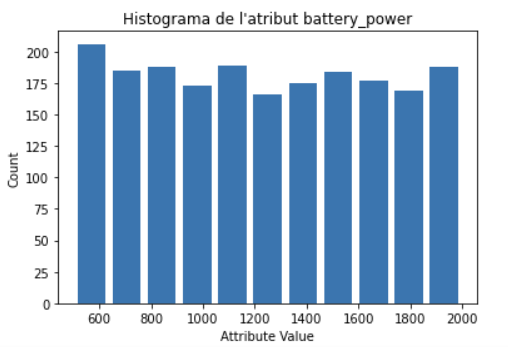
\includegraphics[width=0.3\textwidth]{Histogramas/bt_power.png}}
  \subfloat[\textit{Price Range}]{
    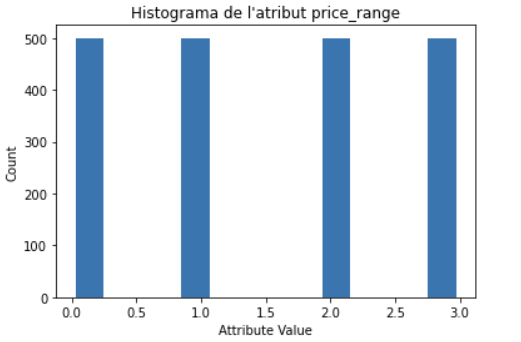
\includegraphics[width=0.3\textwidth]{Histogramas/price_range.png}}
  \subfloat[\textit{Clock Speed}]{
    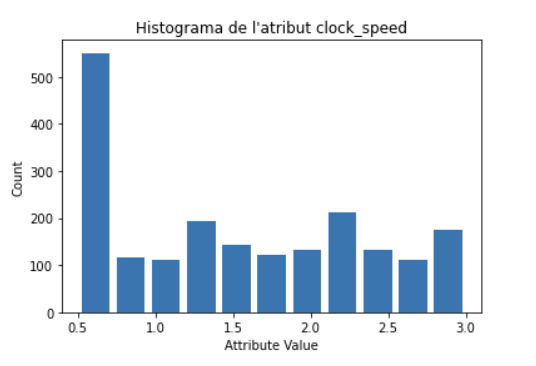
\includegraphics[width=0.3\textwidth]{Histogramas/clock_speed.png}}
    \caption{Mostra dels histogrames generats per l'estudi inicial}
\end{figure}
\hspace{-1.4 em}S'observen les següents característiques dels histogrames\footnote{El conjunt sencer d'histogrames són a \textcolor{blue}{\ref{histogrames}}}:
\begin{itemize}
    \item [$\circ$] L'atribut \textit{price\_range} té el mateix nombre de mostres per a cada valor del seu rang.
    \item [$\circ$] Existeixen atributs que tendeixen a tenir distribucions uniformes.
    \item [$\circ$] Els atributs restants tenen valors molt comuns en comparació de la resta (pel que poden dificultar la classificació)
\end{itemize}
Per a obtenir millors conclusions, es decideix veure les relacions dels atributs representant \textit{price\_range} respecte la resta d'atributs.
\begin{figure}[h]
    \centering
  \subfloat[\textit{Battery Power}]{
    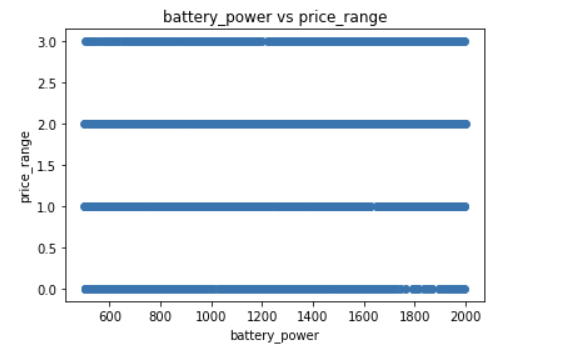
\includegraphics[width=0.3\textwidth]{Scatterplots/battery_price.png}}
  \subfloat[\textit{RAM}]{
    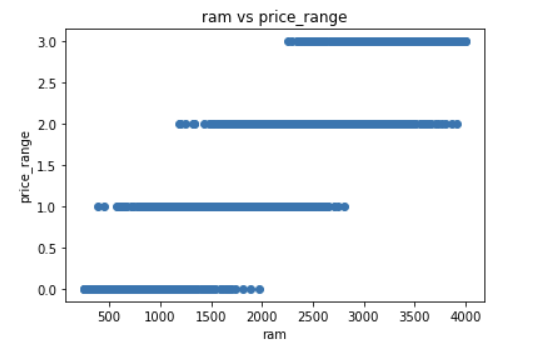
\includegraphics[width=0.3\textwidth]{Scatterplots/ram_price.png}}
  \subfloat[\textit{Clock Speed}]{
    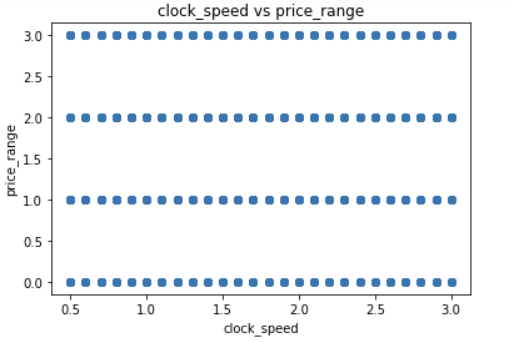
\includegraphics[width=0.3\textwidth]{Scatterplots/clock_price.png}}
    \caption{Mostra dels \textit{scatter-plots} generats per l'estudi inicial}
\end{figure}\\
\hspace{-1.4 em}S'obté dels \textit{scatter-plots} \footnote{El conjunt sencer d'\textit{scatter-plots} són a \textcolor{blue}{\ref{scatter}}} la conclusió que l'únic atribut que sembla tenir bones propietats per a classificar el \textit{price\_range} és el \textit{RAM} ja que mostra una tendencia logística.\\
\newpage
\subsection{Correlació de les variables}\label{correlacio}
S'ha decidit estudiar la correlació entre els atributs que conté la base de dades per tal d'analitzar la importància entre ells per poder trobar els millors paràmetres per classificar i decidir com tractar les incongruències de les dades exposades anteriorment a l'apartat \textcolor{blue}{\ref{exp_dataset}}.

\begin{figure}[h] % Flotante "comun", sin caption, en que irán ambos
\begin{minipage}{7cm} % Minipagina para la tabla. 8 cm de ancho
\begin{center}
    \begin{tabular}{l|l|l}
        \textbf{Atribut} & \textbf{\# afins} & \textbf{Correlació}\\\hline\hline
        \rowcolor{lightapricot}
        Battery\_power & 1 & 0.2007\\\hline
        Blue &  0 & 0.0205\\\hline
        Clock\_speed & 0 & -0.0066\\\hline
        Dual\_sim & 0 & 0.0174\\\hline
        Fc & 1 & 0.0219\\\hline
        Four\_g & 1 & 0.0147\\\hline
        Int\_memory & 0 & 0.0444\\\hline
        M\_dep & 0 & 0.0008 \\\hline
        Mobile\_wt & 0 & -0.0303 \\\hline
        N\_cores & 0 & 0.0043\\\hline
        Pc & 1 & 0.0335\\\hline
        Px\_height & 1 & 0.1488\\\hline
        Px\_width & 1 & 0.1658\\\hline
        \rowcolor{lightapricot}
        RAM &  1 & 0.9170\\\hline
        Sc\_h & 1 & 0.0229\\\hline
        Sc\_w & 1 & 0.0387\\\hline
        Talk\_time & 0 & 0.0218 \\\hline
        Three\_g & 1 & 0.0236\\\hline
        Touch\_screen & 0 & -0.0304 \\\hline
        Wifi & 0 & 0.0187\\\hline
        Price\_range & 2 & 1.0000\\
    \end{tabular}
    Taula 3: Taula d'atributs afins
    \setcounter{table}{2}
    \label{tab:afins}
\end{center}
\end{minipage} % Fin de la minipagina de la tabla
\hspace{2em}
%\hfill % Espacio flexible para separar tabla y figura
\begin{minipage}{7cm} % Minipágina para la figura, 6 cm de ancho
A partir dels resultats obtinguts es pot deduïr que hi existeixen molt poques correlacions entre els atributs, concretament només hi ha dos atributs rellevants que tenen bona correlació amb l'atribut a classificar \textit{prince\_range}.\\\\
A la última columna s'exposen les correlacions dels atributs amb \textit{prince\_range}. Es poden extreure com a variables rellevants: \textit{battery\_power} i \textit{RAM}.
\begin{center}
    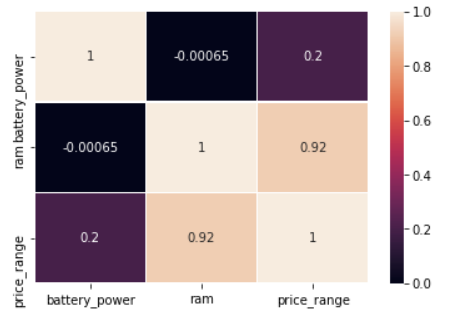
\includegraphics[width=1\textwidth]{corr.png}
    \caption{Correlacions més altes entre els atributs del dataset}
\end{center}

\end{minipage} % Fin de la minipagina que lleva la foto
\end{figure} % Fin del entorno comun. No lleva caption
\hspace{-0.6cm}Es conclou que els atributs que seran utilitzats per a classificar el \textit{prince\_range} són els únics rellevants \footnote{Definim rellevants els atributs que tenen una correlació superior o igual a 0.2} \textit{battery\_power} i \textit{RAM} i, per tant, la resta d'atributs no són importants per a la classificació; pel que no seran tinguts en compte.\\\\
Per aquest motiu, les incongruències trobades a \textcolor{blue}{\ref{exp_dataset}} no cal tenir-les en compte ni tractar-les ja que no hi afecten per a la classificació.
\newpage
\subsection{Anàlisi dels atributs rellevants}\label{analisis_atributs}
Analitzant en més detall les distribucions dels atributs rellevants mencionats anterioment\footnote{Els histogrames dels atributs és troben a \textcolor{blue}{\ref{histogrames}}, així com els \textit{scatter-plots} són a \textcolor{blue}{\ref{scatter}}} s'observa com els dos atributs estan distribuits de forma uniforme entre els diversos rangs de valors.\\ Per altre banda s'intueix com l'atribut \textit{RAM} té una tendència logística (ja explicada i analitzada a \textcolor{blue}{\ref{exp_dataset}}) per contra de l'atribut \textit{battery\_power}, al que no s'intueix cap relació.\\\\
El fet que ambdues variables tinguin distribucions uniformes és una qualitat molt útil a l'hora de classificar ja que permet diferenciar millor les categories en certs rangs (ja que les classes \textit{price\_range} són equiprobables).\\
Tot i així, al no veure una relació directa en la distribució de \textit{battery\_power} respecte a \textit{price\_range} i \textit{RAM}, es va decidir representar les 3 variables per trobar noves relacions que permetessin començar a plantejar models de classificació.
\begin{figure}[h]
    \centering
    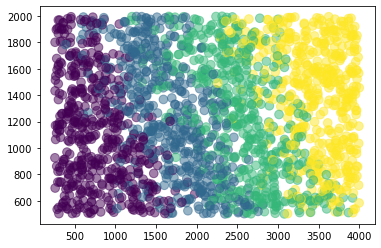
\includegraphics[width=1\textwidth]{colorines.png}
  \caption{\textit{Price\_range} en funció dels paràmetres \textit{RAM} i \textit{battery\_power}.}
  \label{fig:colores}
\end{figure}\\
A partir de la imatge generada\footnote{A la imatge es representa el \textit{price\_range} com a color (essent la gamma de color de més econòmic (lila) a més car (groc)), l'eix $x$ representa la \textit{RAM} i l'eix $y$ representa la \textit{battery\_power}} es pot estimar que existeix una distribució de les dades fàcilment visible.\\
Es mostra també que existeix una certa divisió lineal entre les diferents classes, tot i que aquesta divisió no és completament lineal ja que és bastant difusa, tractant-se així d'una divisió progresiva/continua més que d'una discontinua.\\\\
Malgrat no ser una divisió discreta, s'observa com un model de regressió logística podria classificar de manera bastant precisa el dataset, pel que es començarà estudiant aquest model.

\newpage
\section{Classificació del dataset}\label{classificacio}
\subsection{Logistic Regressor} \label{logistic}
Primerament es provarà un classificador logístic a causa de les observacions fetes anteriorment a \textcolor{blue}{\ref{analisis_atributs}}.
\subsubsection{Estudi de la precisió}
S'inicia l'estudi observant la precisió del model logístic amb paràmetres estàndard.\\
El resultat d'aplicar un regressor logístic per a classificar el dataset de train sencer (sense utilitzar part del mateix per a validar) és:
\begin{figure}[h] % Flotante "comun", sin caption, en que irán ambos
\begin{minipage}{7cm} % Minipagina para la tabla. 8 cm de ancho
\begin{center}
    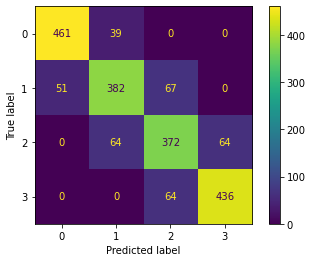
\includegraphics[width=1\textwidth]{ConfMatrix/confusionmatrix_logistic.png}
    \caption{\textit{Confusion matrix} del model logístic estàndard}
\end{center}
\end{minipage} % Fin de la minipagina de la tabla
\hspace{2em}
%\hfill % Espacio flexible para separar tabla y figura
\begin{minipage}{7cm} % Minipágina para la figura, 6 cm de ancho
Es representen en una \textit{confusion matrix} els resultats obtinguts pel classificador Logístic. S'observa com el model no tendeix a confondre classes amb valors molt diferents, si no que, al contrari, tendeix a confondre classes properes entre elles.\\\\
Es dedueix que aquest error és degut a valors propers o pertanyents a les fronteres entre les classes (que són molt difuses ja que es sobreposen).\\\\
Recalcar com en les classes econòmiques (tipus 0) i les classes més cares (tipus 3) tendeix a encertar-ne casi la totalitat de les dades introduïdes que els hi corresponen.
\end{minipage} % Fin de la minipagina que lleva la foto
\end{figure} % Fin del entorno comun. No lleva caption
\\
Calculant l'\textit{accuracy} del model s'obté una precisió del $82.55\%$. Com és una bona predicció s'opta per seguir millorant el model mitjançant un \textit{Cross Validation}.

\subsubsection{Cross Validation}
Al aplicar un \textit{cross validation} (amb 5 subdivisions del dataset) s'obté un resultat \textit{accuracy} de $ 82.55\%$, és a dir, el mateix resultat que sense aplicar el \textit{cross validation} amb tot el dataset. \\\\ 
D'aquest resultat es dedueïx que el regessor que havia singut obtingut inicialment no estava sent \textit{overfitted} i que classifica les classes de telèfons mòbils amb una precisió bastant bona.\\\\
Se segueix l'anàlisis del classificador estudiant la \textit{ROC curve} i la \textit{precission-recall curve} del model.
\newpage
\subsubsection{Anàlisi de la ROC i Precission-Recall Curve} \label{ROC_LOGISTIC}
\begin{figure}[h]
\centering
    \subfloat[\textit{ROC curve}]{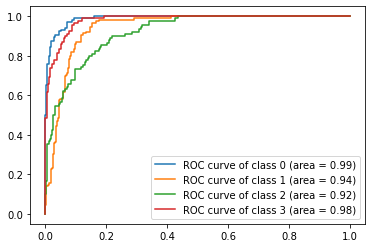
\includegraphics[width = 0.5 \textwidth]{ROCcurve/roc_logistic.png}}
    \subfloat[\textit{Precission-Recall curve}]{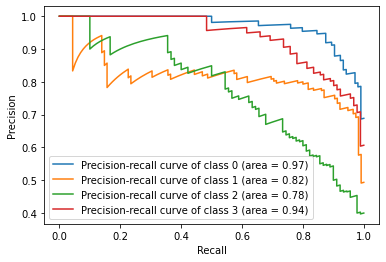
\includegraphics[width = 0.5 \textwidth]{PrecisionRecallCurve/prc_logistic.png}}
    \caption{Corba \textit{ROC} i \textit{Precission-Recall} del model Logístic}
    \label{fig:my_label}
\end{figure}
\hspace{-1.6em}S'observa de la corba \textit{ROC} que l'\textit{accuracy} del model és bona, ja que classifica força bé les diferents classes.\\
Per altra banda, de la corba \textit{Precission-Recall} s'extreu que. a l'hora de classificar les dades, les classes $2$ i $3$ tendeixen a classificar-se de manera errònia, sobretot la clase $2$ que tendeix a confondre's amb la classe $1$ i $3$.\\\\
Per tal de millorar la precisió del model, es cercarà la millor combinació d'hiperparàmetres del model.
\newpage

\subsubsection{Cerca dels millors hiperparàmetres} \label{hiper_para_log}
\begin{figure}[h] % Flotante "comun", sin caption, en que irán ambos
\begin{minipage}{8cm} % Minipagina para la tabla. 8 cm de ancho
 %\rowcolor{lightapricot}
\begin{center} % 0.5-b-lbfgs-l2 0.8275
    \begin{tabular}{l|l}
        \textbf{Paràmetres} & \textbf{Valors} \\\hline\hline
        \multirow{7}{*}{solver} & newton-cg\\
        &\cellcolor{lightapricot}lbfgs\\
        &liblinear\\
        &sag\\
        &saga\\
        &elasticnet\\
        &none\\ \hline
        \multirow{4}{*}{penalty} & l1\\
        & \cellcolor{lightapricot}l2\\
        & elasticnet\\
        & none \\ \hline
        \multirow{5}{*}{intercept\_scaling} & \cellcolor{lightapricot}0.5\\
        & 1\\
        &$\vdots$\\
        & 3.5\\
        & 4\}\\ \hline
        \multirow{5}{*}{weight} & \{1, 1, 1, 1\}\\
        & \{2, 0.5, 0.5, 2\}\\
        & \{0.5, 2, 2, 0.5\}\\
        & \cellcolor{lightapricot}balanced \\
        & None \\
    \end{tabular}
    \caption{Hiperparàmetres model Logístic}
    \label{tab:afins}
\end{center}
\end{minipage} % Fin de la minipagina de la tabla
\hspace{2em}
%\hfill % Espacio flexible para separar tabla y figura
\begin{minipage}{6.5cm} % Minipágina para la figura, 6 cm de ancho
Per a obtenir la millor precisió possible amb el logistic regression s'ha proposat trobar la combinació de paràmetres que maximitzin la \textit{accuracy}.\\ Els paràmetres i valors testejats es mostren a la taula del costat.\\\\
Els resultat de la cerca dels millors hiperparàmetres són els valors remarcats a la taula. Aquests paràmetres permeten obtenir un \textit{accuracy} del $82.75\%$ (tot i que aquest valor pot avegades ser incrementat fins a $83\%$ en alguns casos per fenòmens aleatoris a l'hora de generar el model).\\\\ 
S'observa una milloria no suficientement gran però, degut al poc esforç computacional del programa, és una opció a tenir en compte (ja que dona valors molt correctes i triga poc al executar-se tot i no poder-se millorar molt més el model).
\end{minipage} % Fin de la minipagina que lleva la foto
\end{figure} % Fin del entorno comun. No lleva caption
\hspace{-1.6em}Seguidament, es procedeix a analitzar les corbes \textit{ROC} i \textit{Precision-Recall} del model amb els millors hiperparàmetres:\\
\vspace{-2em}
\begin{figure}[h]
\centering
    \subfloat[\textit{ROC curve}]{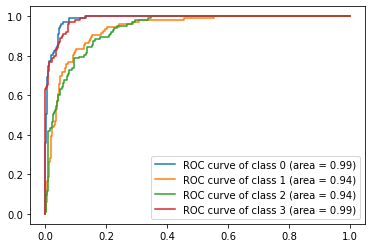
\includegraphics[width = 0.4 \textwidth]{BetterROC/ultim_roc_logistic.png}}
    \subfloat[\textit{Precission-Recall curve}]{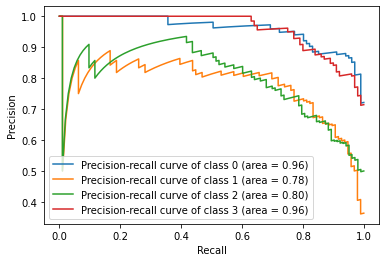
\includegraphics[width = 0.4 \textwidth]{BetterPrecision/ultim_precision_logistic.png}}
    \caption{Corba \textit{ROC} i \textit{Precission-Recall} del millor model Logístic}
    \label{fig:my_label}
\end{figure}\\
S'observa com les corbes han cambiat respecte a les obtingudes a \textcolor{blue}{\ref{ROC_LOGISTIC}}, més concretament es pot apreciar que la corba \textit{ROC} ha millorat en totes les classes.\\
D'altra banda \textit{Precission-Recall} al principi les classes $1$ i $2$ empitjoren però millora breument al final. Tot i així, el valor que obté la classe $2$ no és millor que anteriorment.\\\\
Al millorar les dades obtingudes (de l'\textit{accuracy} i les corbes \textit{ROC} i \textit{Precision-Recall}), es conclou que aquest model és eficaç i que s'emprarà per comparar amb altres models.
\newpage
\subsubsection{Resultats del classificador}\label{zona_logistic}
Finalment, s'obté la \textit{zona de decisió} del classificador logístic amb els millors hiperparàmetres\footnote{Els hiperparàmetres que milloren el classificador són explicats a \textcolor{blue}{\ref{hiper_para_log}}} obtinguts:\\
\begin{figure}[h]
    \centering
    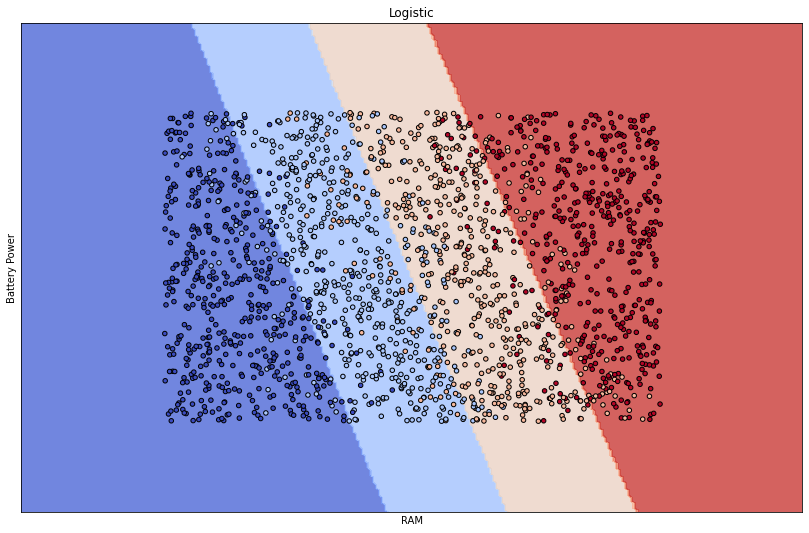
\includegraphics[width = 1\textwidth]{ZonasModelos/zona_logistic.png}
    \caption{Zona de decisió del millor model logístic trobat}
    \label{fig:my_label}
\end{figure}\\
S'observa com el model senyala de manera intuïtiva les divisions entre les classes, tot i així, algunes dades que hi són a les fronteres es troben mal etiquetades.\\\\
No obstant, aquests casos són escassos i, per tant, són insuficients com per a alterar el classificador.\\\
Es dedueïx que la precisió del model no podrà superar un cert umbral degut a aquest valor i, intuïm, que aquest serà inferior o igual a $90\%$. \\\\
Es provaran altres models de classificació per a intentar arribar aquest umbral (si existeix o superar-lo en cas contrari).
\newpage


\subsection{K-Nearest Neighbors}\label{KNN}
\subsubsection{Estudi de la precisió}
Es continua l'estudi observant la precisió del model KNN amb paràmetres estàndards, ja que al tractar-se d'un dataset amb dades molt compactes podria obtenir bons resultats.\\
El resultat d'aplicar aquest model per a classificar el dataset de train sencer (sense utilitzar part del mateix per a validar) és:
\begin{figure}[h] % Flotante "comun", sin caption, en que irán ambos
\begin{minipage}{7cm} % Minipagina para la tabla. 8 cm de ancho
\begin{center}
    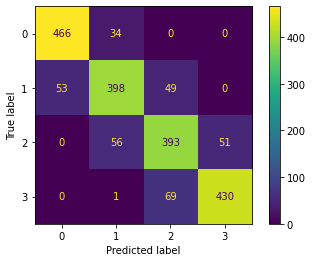
\includegraphics[width=1\textwidth]{ConfMatrix/confusionmatrix_KNN.png}
    \caption{\textit{Confusion matrix} del K-Nearest Neighbors}
\end{center}
\end{minipage} % Fin de la minipagina de la tabla
\hspace{2em}
%\hfill % Espacio flexible para separar tabla y figura
\begin{minipage}{7cm} % Minipágina para la figura, 6 cm de ancho
A la figura s'identifiquen en una \textit{confusion matrix} els resultats obtinguts pel classificador. S'observa com el model tendeix a confondre classes properes entre elles, mentre que amb classes molt separades (com és el cas de la 0 i la 3) no té cap tipus de confusió.\\\\
Es dedueix que els errors es deuen a valors propers o pertanyents a les fronteres entre les classes (que són molt difuses ja que es sobreposen).\\\\
Cal recalcar que el comportament del model és molt similar al model logístic ja estudiat abans, pel que es pot calcular que la tendència serà similar en els següents models que seràn provats.
\end{minipage} % Fin de la minipagina que lleva la foto
\end{figure} % Fin del entorno comun. No lleva caption
\\
Calculant l'\textit{accuracy} del model s'obté una precisió del $84.35\%$. Com és una bona predicció s'opta per seguir millorant el model mitjançant un \textit{Cross Validation}.


\subsubsection{Cross Validation}
Al aplicar un cross validation (amb 5 subdivisions del dataset) s’obté un resultat \textit{accuracy}
de $78.5\%$. Si bé és inferior al valor resultant inicialment, aquest comportament es pot explicar de dues maneres:
\begin{itemize}
    \item El model està \textit{overfitted}.
    \item El model requeria de més dades per a millorar la predicció.
\end{itemize}
No es pot assegurar que el model hagi estat \textit{overfitted}, ja que al tractar-se d'un model KNN, requereix de moltes dades per a funcionar i, al reduïr el \textit{train dataset} per a obtenir un \textit{test dataset}, es podria donar una disminució de la precisió.\\
Es procedeix doncs a estudiar la precisió del model mitjançant les curves \textit{ROC} i \textit{Precision-Recall}.
\newpage
\subsubsection{Anàlisi de la ROC i Precission-Recall Curve} \label{ROC_KNN}
\begin{figure}[h]
\centering
    \subfloat[\textit{ROC curve}]{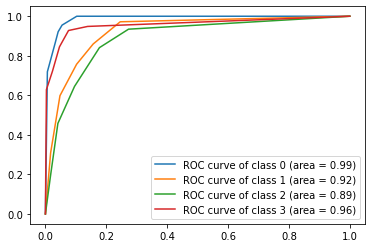
\includegraphics[width = 0.5 \textwidth]{ROCcurve/roc_knn.png}}
    \subfloat[\textit{Precission-Recall curve}]{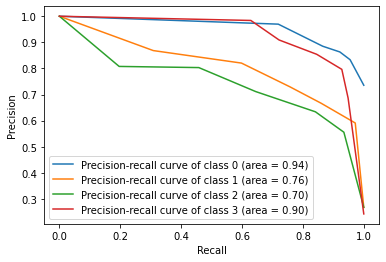
\includegraphics[width = 0.5 \textwidth]{PrecisionRecallCurve/prc_knn.png}}
    \caption{Corba \textit{ROC} i \textit{Precission-Recall} del model KNN}
    \label{fig:my_label}
\end{figure}
\hspace{-1.6em}Es pot apreciar de la corba \textit{ROC} que l'\textit{accuracy} del model és bona, ja que classifica força bé les diferents classes. \\
Per altra banda, de la corba \textit{Precission-Recall} s'extreu que, a l'hora de classificar les dades, les classes 0 i 3 es classifiquen de manera correcta en la majoria dels casos. En canvi, les classes 1 i 2 tendeixen a classificar-se de manera errònia, sobretot la classe $2$, que tendeix a confondre's amb la classe $1$.\\\\
Destacar que les corbes no són tan bones com al model Logístic (\textcolor{blue}{\ref{ROC_LOGISTIC}}). Tot i així, el rang de millora és bastant més elevat que amb el logístic, pel que es cercaran els millors hiperparàmetres per tal de millorar el model el màxim possible. 
\newpage
\subsubsection{Cerca dels millors hiperparàmetres}\label{millorsknn}
\begin{figure}[h] % Flotante "comun", sin caption, en que irán ambos
\begin{minipage}{8cm} % Minipagina para la tabla. 8 cm de ancho
 %\rowcolor{lightapricot}
\begin{center} % 0.5-b-lbfgs-l2 0.8275
    \begin{tabular}{l|l}
        \textbf{Paràmetres} & \textbf{Valors} \\\hline\hline
        \multirow{2}{*}{weights} & \cellcolor{lightapricot}uniform\\
        &distance\\\hline
        \multirow{4}{*}{algorithm} & \cellcolor{lightapricot}auto\\
        & ball\_tree \\ 
        & kd\_tree\\
        & brute\\ \hline
        \multirow{3}{*}{p} & \cellcolor{lightapricot}{1\\
        &$\vdots$\\
        & 10}\\ \hline
        \multirow{5}{*}{n\_neighbors} & 1\\
        & $\vdots$\\
        & \cellcolor{lightapricot}11\\
        & $\vdots$\\
        & 30 \\
    \end{tabular}
    \caption{Hiperparàmetres model KNN}
    \label{tab:afins}
\end{center}
\end{minipage} % Fin de la minipagina de la tabla
\hspace{2em}
%\hfill % Espacio flexible para separar tabla y figura
\begin{minipage}{6.5cm} % Minipágina para la figura, 6 cm de ancho
Per a obtenir la millor precisió possible amb el KNN s'ha proposat trobar la combinació de paràmetres que maximitzin la \textit{accuracy}.\\ Els paràmetres i valors testejats es mostren a la taula del costat.\\\\
Els resultat de la cerca dels millors hiperparàmetres són els valors remarcats a la taula. Aquest paràmetres permeten obtenir un \textit{accuracy} del $81.5\%$ (tot i que aquest valor, en alguns casos, es pot incrementar fins a $83\%$ en alguns casos per fenòmens aleatoris a l'hora de generar el model).\\\\ 

\end{minipage} % Fin de la minipagina que lleva la foto
\end{figure} % Fin del entorno comun. No lleva caption
\hspace{-1.6em}S'observa una milloria però no n'és suficient en comparació al regressor logístic (\textcolor{blue}{\ref{hiper_para_log}}.\\
Com el model té un cost computacional baix i un percentatge d'encert semblant al logístic, es manté el model com a vàlid i s'analitzen les seves corbes \textit{ROC} i \textit{Precision-Recall}.\\
\hspace{-1.6em}S'analitzen ara les corbes \textit{ROC} i \textit{Precision-Recall} del model amb els millors hiperparàmetres:\\
\vspace{-2em}
\begin{figure}[h]
\centering
    \subfloat[\textit{ROC curve}]{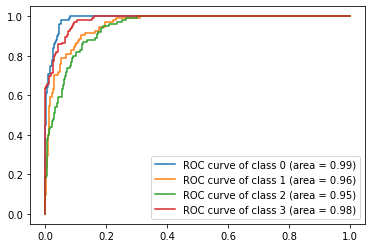
\includegraphics[width = 0.4 \textwidth]{BetterROC/ultim_roc_knn.png}}
    \subfloat[\textit{Precission-Recall curve}]{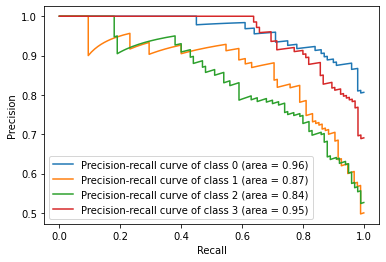
\includegraphics[width = 0.4 \textwidth]{BetterPrecision/ultim_precision_knn.png}}
    \caption{Corba \textit{ROC} i \textit{Precission-Recall} del millor model KNN}
    \label{fig:my_label}
\end{figure}\\
S'observa com les corbes han cambiat respecte a les obtingudes a \textcolor{blue}{\ref{ROC_LOGISTIC}}, concretament com les dues corbes ha millorat en totes les classes.
No obstant, s'observa el següent:
\begin{itemize}
    \item La \textit{Recall} i \textit{Precission} han millorat en valor en totes
    \item Les classes $1$ i $2$ inicialment tenen bastants errors, peró desprès milloren substancialment per a terminar oferint millors resultats
    \item Els valors son força semblants al Logístic, però no el suficient com per a classificar igual, pel que surgeix la idea de combinar els models en un ensemble. 
\end{itemize}
\newpage

\subsubsection{Resultats del classificador}\label{zona_knn}
Finalment, s'obté la \textit{zona de decisió} del classificador KNN amb els millors hiperparàmetres\footnote{Els hiperparàmetres que milloren el classificador són explicats a \textcolor{blue}{\ref{millorsknn}}} obtinguts:\\
\begin{figure}[h]
    \centering
    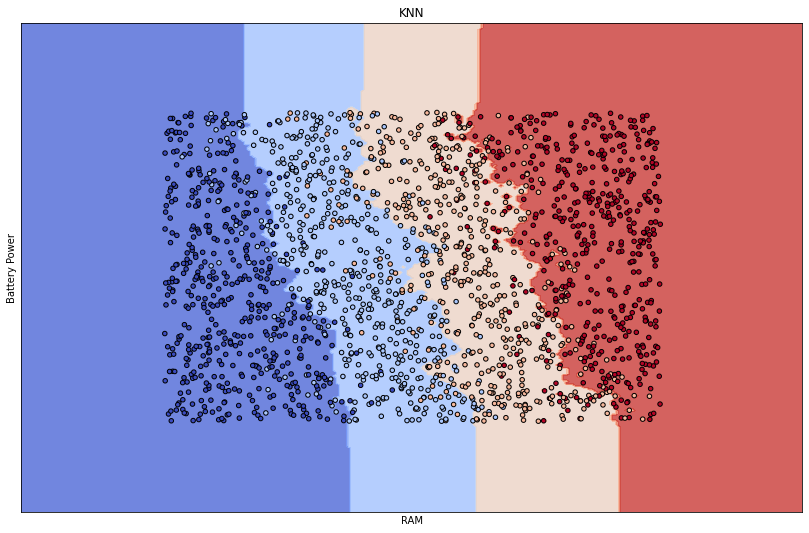
\includegraphics[width = 1\textwidth]{ZonasModelos/zona_knn.png}
    \caption{Zona de decisió del millor model KNN trobat}
    \label{fig:my_label}
\end{figure}\\
S'observa com el model senyala de manera difussa les divisions entre les classes, tot i així, algunes dades es troben mal etiquetades i les fronteres de decissió no son clares i obtenen formes peculiars.\\\\
Aquest comportament (com el de crear regions de tipus de classes on clarament predomina un tipus diferent) fa que aquest mètode no pugui ser molt util en clasifficar dades noves entrants de manera eficaç.\\\\
Com el mètode obte prediccions semblants al Logístic i té una precisió decent, es manté el model KNN per a implementar-lo en clasificador de tipus ensemble.
\newpage



\subsection{Support Vector Classification}\label{SVC}
\subsubsection{Estudi de la precisió}
Es continua l'estudi observant la precisió del model SVC amb paràmetres estàndards, ja que es considera que (al dividir zones per fronteres rectes amb toleràncies) podria donar bons resultats.\\
El resultat d'aplicar aquest model per a classificar el dataset de train sencer (sense utilitzar part del mateix per a validar) és:
\begin{figure}[h] % Flotante "comun", sin caption, en que irán ambos
\begin{minipage}{7cm} % Minipagina para la tabla. 8 cm de ancho
\begin{center}
    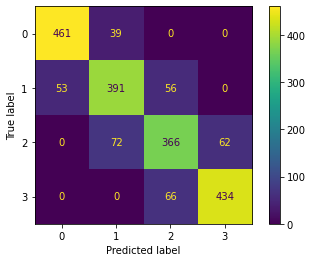
\includegraphics[width=1\textwidth]{ConfMatrix/confusionmatrix_svc.png}
    \caption{\textit{Confusion matrix} del SVC}
\end{center}
\end{minipage} % Fin de la minipagina de la tabla
\hspace{2em}
%\hfill % Espacio flexible para separar tabla y figura
\begin{minipage}{7cm} % Minipágina para la figura, 6 cm de ancho
A la figura s'identifiquen en una \textit{confusion matrix} els resultats obtinguts pel classificador. S'observa com el model obté resultats molt similars als del model logístic i del model KNN (\textcolor{blue}{\ref{zona_logistic}} i \textcolor{blue}{\ref{zona_knn}} respectivament).\\\\
La única diferencia significativa del model es que tendeix a infravalorar el tipus de classe (tendint a catalogar un tipus inferior més que superior en cas de classificar-lo de manera erronia).\\\\
Si bé no es un comportament desitjat pel classificador (ja que ha de ser el més precís possible), torna a proporcionar la idea de crear un ensemble de model.
\end{minipage} % Fin de la minipagina que lleva la foto
\end{figure} % Fin del entorno comun. No lleva caption
\\
Calculant l'\textit{accuracy} del model s'obté una precisió del $82.6\%$. Com és una bona predicció s'opta per seguir millorant el model mitjançant un \textit{Cross Validation}.


\subsubsection{Cross Validation}
Al aplicar un cross validation (amb 5 subdivisions del dataset) s’obté un resultat \textit{accuracy}
de $82.4\%$. Si bé és inferior al valor resultant inicial, aquest és molt proper.\\\\ 
No es pot assegurar que el model inicial hagi estat \textit{overfitted}, peró al obtenir una precisió tan similar (i alt) es pot intuïr que realment pot tractar-se d'un model eficient a l'hora de classificar les dades.\\\\
Es procedeix doncs a estudiar la precisió del model mitjançant les curves \textit{ROC} i \textit{Precision-Recall}.
\newpage
\subsubsection{Anàlisi de la ROC i Precission-Recall Curve} \label{ROC_SVC}
\begin{figure}[h]
\centering
    \subfloat[\textit{ROC curve}]{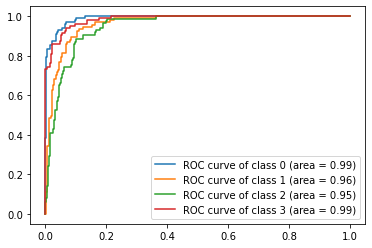
\includegraphics[width = 0.5 \textwidth]{ROCcurve/roc_svc.png}}
    \subfloat[\textit{Precission-Recall curve}]{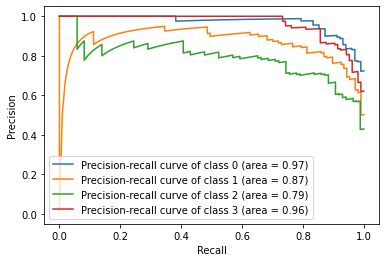
\includegraphics[width = 0.5 \textwidth]{PrecisionRecallCurve/prc_svc.png}}
    \caption{Corba \textit{ROC} i \textit{Precission-Recall} del model SVC}
    \label{fig:my_label}
\end{figure}
\hspace{-1.6em}Es pot apreciar de la corba \textit{ROC} que l'\textit{accuracy} del model és bona, ja que classifica força bé les diferents classes. \\
Per altra banda, de la corba \textit{Precission-Recall} s'extreu un comportament similar al del model logístic (\textcolor{blue}{\ref{ROC_LOGISTIC}}). \\
\\
Recalcar que aquest model té una pitjor precisió inicial (respecte a la classe 1) que la resta de models, pel que la cerca de hiperparàmetres no només es centrarà en la millora de la precisió, sino que també s'enfocarà en millorar la precisió de la classificació de la clase de tipus $3$.
\newpage
\subsubsection{Cerca dels millors hiperparàmetres} \label{hiper_par_SVC}
\begin{figure}[h] % Flotante "comun", sin caption, en que irán ambos
\begin{minipage}{8cm} % Minipagina para la tabla. 8 cm de ancho
 %\rowcolor{lightapricot}
\begin{center} % 0.5-b-lbfgs-l2 0.8275
    \begin{tabular}{l|l}
        \textbf{Paràmetres} & \textbf{Valors} \\\hline\hline
        \multirow{4}{*}{kernel} & linear\\
        &poly\\
        &\cellcolor{lightapricot}rbf\\
        &sigmoid\\ \hline
        \multirow{2}{*}{gamma} & \cellcolor{lightapricot}scale\\
        & auto\\
    \end{tabular}
    \caption{Hiperparàmetres model KNN}
    \label{tab:afins}
\end{center}
\end{minipage} % Fin de la minipagina de la tabla
\hspace{2em}
%\hfill % Espacio flexible para separar tabla y figura
\begin{minipage}{6.5cm} % Minipágina para la figura, 6 cm de ancho
Per a obtenir la millor precisió possible amb el SVC s'ha proposat trobar la combinació de paràmetres que maximitzin la \textit{accuracy}.\\\\ Els paràmetres i valors testejats es mostren a la taula del costat.\\\\

\end{minipage} % Fin de la minipagina que lleva la foto
\end{figure} % Fin del entorno comun. No lleva caption
\hspace{-1.6em}Els resultats de la cerca dels millors hiperparàmetres són els valors remarcats a la taula. Aquests paràmetres permeten obtenir un \textit{accuracy} del $84\%$ (tot i que aquest valor pot oscil·lar entre $82\%$ i $85\%$ per fenòmens aleatoris).\\\\ S'observa una milloria substancial en comparació al regressor logístic (\textcolor{blue}{\ref{hiper_para_log}}) i al anterior model KNN (\textcolor{blue}{\ref{millorsknn}}).\\
Com el model té un cost computacional baix i un percentatge d'encert semblant al logístic, es manté el model com a vàlid i s'analitzen les seves corbes \textit{ROC} i \textit{Precision-Recall}.\\
\hspace{-1.6em}S'analitzen ara les corbes \textit{ROC} i \textit{Precision-Recall} del model amb els millors hiperparàmetres:\\
\vspace{-2em}
\begin{figure}[h]
\centering
    \subfloat[\textit{ROC curve}]{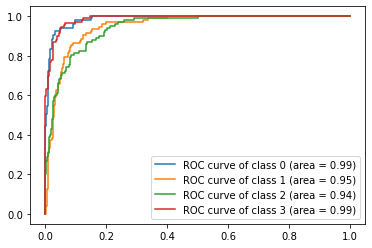
\includegraphics[width = 0.4 \textwidth]{BetterROC/ultim_roc_svc.png}}
    \subfloat[\textit{Precission-Recall curve}]{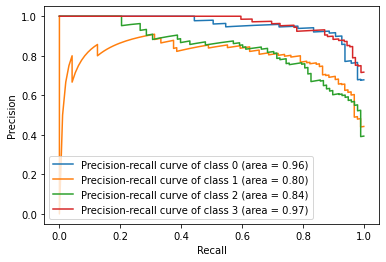
\includegraphics[width = 0.4 \textwidth]{BetterPrecision/ultim_precision_svc.png}}
    \caption{Corba \textit{ROC} i \textit{Precission-Recall} del millor model SVC}
    \label{fig:my_label}
\end{figure}\\
S'observa com les corbes no han cambiat respecte a les obtingudes a \textcolor{blue}{\ref{ROC_SVC}}, 
No obstant, s'observa el següent:
\begin{itemize}
    \item La \textit{Recall} i \textit{Precission} ha empitjorat en 3 de les 4 classes
    \item La classe $1$ conté inicialment bastants errors peró desprès millora substancialment com per a obtenir valors similars a la gràfica del model sense cerca d'hiperparàmetres.
    \item Els valors segueixen sent força semblants al Logìstic, però no el suficient com per a classificar igual, pel que es manté la idea de combinar els models en un ensemble. 
\end{itemize}
\newpage

\subsubsection{Resultats del classificador}\label{zona_svc}
Finalment, s'obté la \textit{zona de decisió} del classificador SVC amb els millors hiperparàmetres\footnote{Els hiperparàmetres que milloren el classificador són explicats a \textcolor{blue}{\ref{hiper_par_SVC}}} obtinguts:\\
\begin{figure}[h]
    \centering
    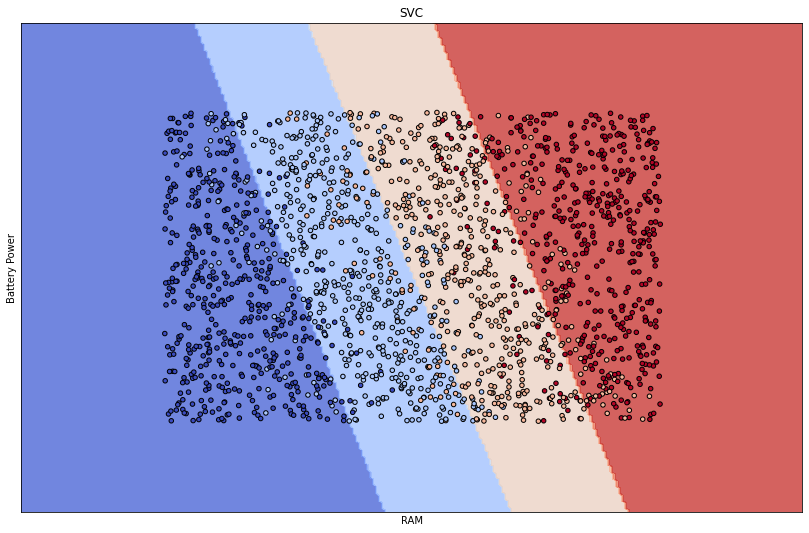
\includegraphics[width = 1\textwidth]{ZonasModelos/zona_svc.png}
    \caption{Zona de decisió del millor model SVC trobat}
    \label{fig:my_label}
\end{figure}\\
S'observa com el model senyala de manera similar al regressor logístic les divisions entre les classes, tot i així, algunes dades es troben mal etiquetades degut a les fronteres tan difuses de les dades.\\\\
Com el mètode obté prediccions semblants al Logístic i té una precisió eficaç (depenen d'un cert factor aleatori), es manté el model SVC com a un molt bon candidat i també per a implementar-lo en classificador de tipus ensemble.
\newpage
\subsubsection{Model LinearSVC}\label{zona_linearsvc}
Al haver observat que un dels hiperparàmetres del model SVC trobat que fa millorar la predicció, és el paràmetre de \textit{Linear}\footnote{Hiperparàmetres explicats a \textcolor{blue}{\ref{hiper_par_SVC}}}, s'ha decidit estudiar el comportament del model LinearSVC de manera exprés (estudiant directament els hiperparàmetres\footnote{En cas de volver consultar-los, revisar el codi entregat conjuntament amb aquesta memòria} i la zona de decisió) amb el propòsit d'obtenir un millor resultat.\\
A continuació es presenta la zona de decisió:
\begin{figure}[h]
    \centering
    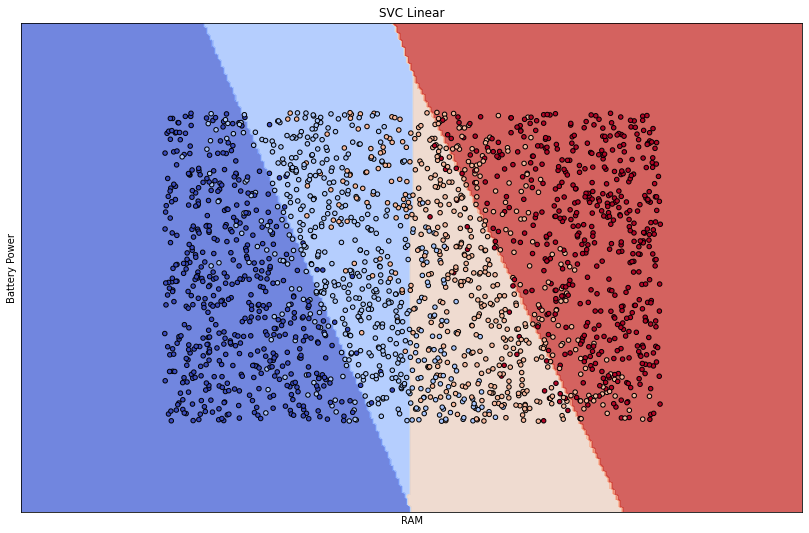
\includegraphics[width = 0.7\textwidth]{ZonasModelos/zona_linear.png}
    \caption{Zona de decisió del millor model LinearSVC}
    \label{fig:my_label}
\end{figure}\\
Executant el model, obtenim una \textit{accuracy} del $76.25\%$ que, en comparació amb la obtinguda amb el millor model SVC, no resulta prou bona.\\\\
Aquest resultat s'explica per com es divideixen les zones de decisió a aquest model, ja que divideix les classes $1$ i $2$ d'una manera poc intuïtiva i de forma que moltes dades s'etiqueten de forma errònia.\\\\
A causa de tot això, es conclou que es tracta d'un mal model.
\newpage


\subsection{Decision Tree Classificator}\label{TREE}
\subsubsection{Estudi de la precisió}
Es continua l'estudi observant la precisió del model \textit{DecisionTreeClassifier} amb paràmetres estàndard, aquesta decisió es pren per intentar tornar a dividir el model en línies rectes, però ara mitjançant escalonaments.\\
El resultat d'aplicar aquest model per a classificar el dataset de train sencer (sense utilitzar part del mateix per a validar) és:
\begin{figure}[h] % Flotante "comun", sin caption, en que irán ambos
\begin{minipage}{7cm} % Minipagina para la tabla. 8 cm de ancho
\begin{center}
    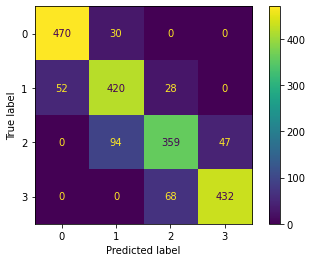
\includegraphics[width=1\textwidth]{ConfMatrix/confusionmatrix_decisiontree.png}
    \caption{\textit{Confusion matrix} del \textit{DecisionTreeClassifier}}
\end{center}
\end{minipage} % Fin de la minipagina de la tabla
\hspace{2em}
%\hfill % Espacio flexible para separar tabla y figura
\begin{minipage}{7cm} % Minipágina para la figura, 6 cm de ancho
A la figura s'observen en una \textit{confusion matrix} els resultats obtinguts pel classificador. S'observa com el model tendeix a un comportament similar al del model SVC (\textcolor{blue}{\ref{SVC}}), ja que tendeix a infraestimar les classes.\\\\
Cal recalcar que la classe de tipus $2$ té bastants problemes a l'hora d'etiquetar-la, ja que és el model que menys etiquetes encerta de les de tipus $2$.\\\\
Aquest comportament n'indica que el model podria no ser suficientment adien;, tot i així, s'opta per millorar-lo, amb la intenció d'esbrinar algun nou model que pugui oferir millors resultats
\end{minipage} % Fin de la minipagina que lleva la foto
\end{figure} % Fin del entorno comun. No lleva caption
\\
Calculant l'\textit{accuracy} del model s'obté una precisió del $84.05\%$. Com és una bona predicció s'opta per seguir millorant el model mitjançant un \textit{Cross Validation}.

\subsubsection{Cross Validation}
Al aplicar un cross validation\footnote{El \textit{K-Fold} del \textit{Cross Validation} és igual que als anterior $K=5$, pel que s'omet i s'ometrà en els futurs anàlisis dels models} s’obté un resultat accuracy
de $79.7\%$, el qual és un bon resultat, i, com en va passar al model KNN (\textcolor{blue}{\ref{KNN}}) la mateixa precisió que sense el \textit{Cross Validation}. \\ Per tant, s'arriba a la mateixa conclusió i es continua amb l'anàlisi del model mitjançant un estudi de les corbes \textit{ROC} i \textit{Precision-Recall}.
\newpage
\subsubsection{Anàlisi de la ROC i Precission-Recall Curve} \label{ROC_DECISIONTREE}
\begin{figure}[h]
\centering
    \subfloat[\textit{ROC curve}]{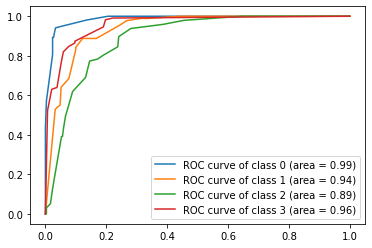
\includegraphics[width = 0.5 \textwidth]{ROCcurve/roc_decisiontree.png}}
    \subfloat[\textit{Precission-Recall curve}]{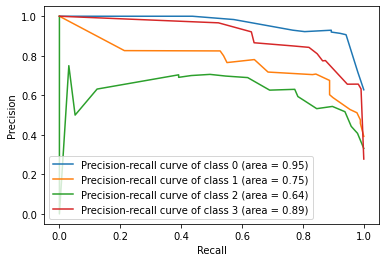
\includegraphics[width = 0.5 \textwidth]{PrecisionRecallCurve/prc_decisiontri.png}}
    \caption{Corba \textit{ROC} i \textit{Precission-Recall} del model DecisionTree}
    \label{fig:my_label}
\end{figure}
\hspace{-1.6em}S'observa de la corba \textit{ROC} que l'\textit{accuracy} del model és bona, ja que classifica força bé les diferents classes. Tot i així, els valors que s'obtenen no són del tot adients en comparació amb altres models com el Logístic o el SVC (\textcolor{blue}{\ref{logistic}} i \textcolor{blue}{\ref{SVC}} respectivament).\\\\
Per altra banda, de la corba \textit{Precission-Recall} s'extreu que, a l'hora de classificar les dades, les classes 1 i 2 es classifiquen de manera errònia. Aquesta situació és especialment visible a la classe $2$, que obté un valor de \textit{Precission-Recall} molt baix per comparació a la resta de models provats.
Es buscarà millorar el classificador mitjançant una cerca dels hiperparàmetres que permetin millorar la precisió del model així com la classificació de les dades amb etiqueta de valor $2$.
\newpage
\subsubsection{Cerca dels millors hiperparàmetres}
\label{hiper_decisiontree}
\begin{figure}[h] % Flotante "comun", sin caption, en que irán ambos
\begin{minipage}{8cm} % Minipagina para la tabla. 8 cm de ancho
 %\rowcolor{lightapricot}
\begin{center} % 0.5-b-lbfgs-l2 0.8275
    \begin{tabular}{l|l}
        \textbf{Paràmetres} & \textbf{Valors} \\\hline\hline
        \multirow{2}{*}{criterion} & gini\\
        &\cellcolor{lightapricot}entropy\\ \hline
        \multirow{2}{*}{splitter} & \cellcolor{lightapricot}best\\
        & random \\ \hline
        \multirow{4}{*}{max\_features} & \cellcolor{lightapricot}sqrt\\
        & log2 \\ & random \\ & None \\ \hline
        \multirow{5}{*}{max\_depth} & 2\\
        & $\vdots$ \\ 
        & \cellcolor{lightapricot}5 \\ 
        & $\vdots$  \\ 
        & 30 \\\hline
        \multirow{4}{*}{min\_samples\_split} & \cellcolor{lightapricot}2\\
        & $\vdots$ \\ 
        & 10 \\
    \end{tabular}
    \caption{Hiperparàmetres model Decision Tree}
    \label{tab:afins}
\end{center}
\end{minipage} % Fin de la minipagina de la tabla
\hspace{2em}
%\hfill % Espacio flexible para separar tabla y figura
\begin{minipage}{6.5cm} % Minipágina para la figura, 6 cm de ancho
Per a obtenir la millor precisió possible amb el DecisionTree s'ha proposat trobar la combinació de paràmetres que maximitzin la \textit{accuracy}.\\ Els paràmetres i valors testejats es mostren a la taula del costat.\\\\
Els resultats de la cerca dels millors hiperparàmetres són els valors remarcats a la taula. Aquests paràmetres permeten obtenir un \textit{accuracy} del $81.5\%$.\\\\ 
S'observa una milloria substancialment gran, però en tot cas insuficient com per a competir amb el model logistic i SVC (\textcolor{blue}{\ref{logistic}} i \textcolor{blue}{\ref{SVC}} respectivament).\\\\
Precedim a estudiar les corbes \textit{ROC} i \textit{Precision-Recall}.
\end{minipage} % Fin de la minipagina que lleva la foto
\end{figure} % Fin del entorno comun. No lleva caption
\begin{figure}[h]
\centering
    \subfloat[\textit{ROC curve}]{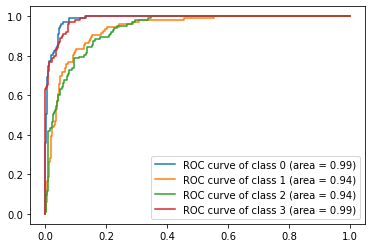
\includegraphics[width = 0.4 \textwidth]{BetterROC/ultim_roc_logistic.png}}
    \subfloat[\textit{Precission-Recall curve}]{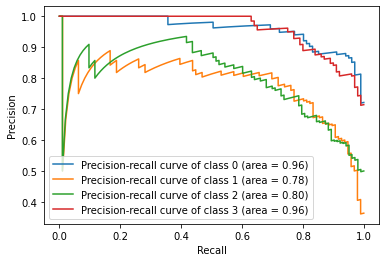
\includegraphics[width = 0.4 \textwidth]{BetterPrecision/ultim_precision_logistic.png}}
    \caption{Corba \textit{ROC} i \textit{Precission-Recall} del millor model Logístic}
    \label{fig:my_label}
\end{figure}\\
S'observa com les corbes han cambiat dràsticament respecte a les obtingudes.\\\\
Tot i així, les característiques de les corbes són força similars al models ja observat del KNN (\textcolor{blue}{\ref{KNN}}), pel que no es creu necessari utilitzar aquest mètode degut a la ineficiència a l'hora de classificar respecte dels mètodes que hem utilitzar al comparar-lo.\\\\
Per altra banda, al millorar les dades obtingudes (de l'\textit{accuracy} i les corbes \textit{ROC} i \textit{Precision-Recall}), es conclou que aquest model pot servir amb mètodes d'\textit{ensemble} per a millorar la seva predicció.
\newpage
\subsubsection{Resultats del classificador}\label{zona_decisiontree}
Finalment, s'obté la \textit{zona de decisió} del classificador amb els millors hiperparàmetres\footnote{Els hiperparàmetres que milloren el classificador són explicats a \textcolor{blue}{\ref{hiper_decisiontree}}} obtinguts:\\
\begin{figure}[h]
    \centering
    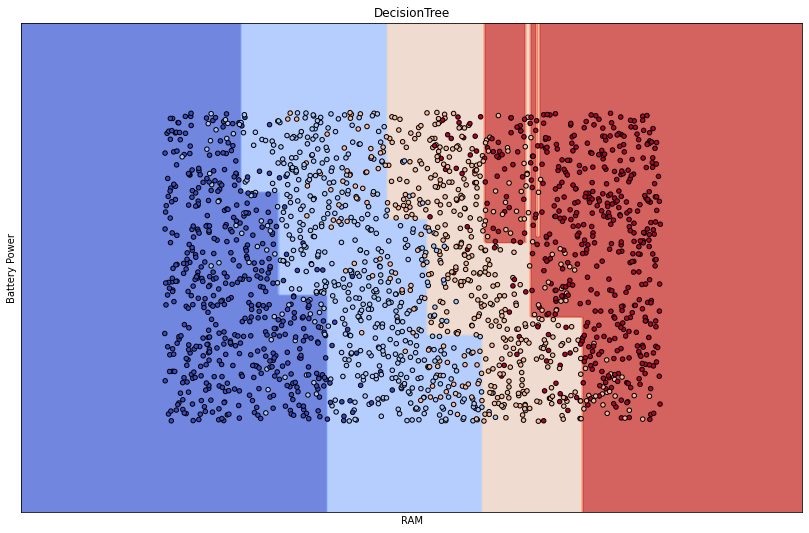
\includegraphics[width = 1\textwidth]{ZonasModelos/zona_decision.png}
    \caption{Zona de decisió del millor model \textit{Decision Tree} trobat}
    \label{fig:my_label}
\end{figure}\\
S'observa com les fronteres de decisió no son intuïtives i que moltes dades no s'han etiquetat correctament.\\\\
Confirmem la conclusió de desestimar el mètode i és proposa estudiar-ne un ensemble de DecisionTree.
\newpage


\subsection{Random Forest Classificator}\label{random}
\subsubsection{Estudi de la precisió}
Es continua l'estudi observant la precisió del \textit{RandomForest} amb paràmetres estàndard, ja que amb els resultats anterior s'intueix que es poden obtenir bons resultats.\\
El resultat d'aplicar aquest model per a classificar el dataset de train sencer (sense utilitzar part del mateix per a validar) és:
\begin{figure}[h] % Flotante "comun", sin caption, en que irán ambos
\begin{minipage}{7cm} % Minipagina para la tabla. 8 cm de ancho
\begin{center}
    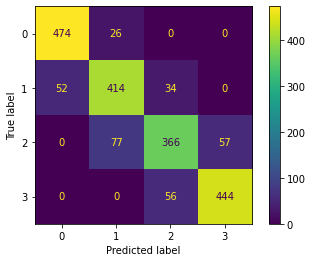
\includegraphics[width=1\textwidth]{ConfMatrix/confusionmatrix_random.png}
    \caption{\textit{Confusion matrix} del RandomForestClassifier}
\end{center}
\end{minipage} % Fin de la minipagina de la tabla
\hspace{2em}
%\hfill % Espacio flexible para separar tabla y figura
\begin{minipage}{7cm} % Minipágina para la figura, 6 cm de ancho
A la figura s'observen en una \textit{confusion matrix} els resultats obtinguts pel classificador. S'observa com el model tendeix a obtenir els mateixos resultats que el DecisionTree (\textcolor{blue}{\ref{TREE}}), efecte que té sentit al tractar-se d'un ensemble de DecisionTrees.\\\\
Com que els resultats són similars als Decision tree, però al executar-se s'obté una \textit{accuracy} del model $84.9\%$, és a dir, una molt bona precisió. Per tant, s'opta per seguir millorant el model mitjançant un \textit{Cross Validation}.
\end{minipage} % Fin de la minipagina que lleva la foto
\end{figure} % Fin del entorno comun. No lleva caption


\subsubsection{Cross Validation}
Al aplicar un cross validation  s’obté un resultat accuracy
de $80.75\%$. Com que la precisió ha disminuït sustancialment, es conclou que el model estaba \textit{overfitted} pel que caldra tenir en cura l'introducció de les dades i la gestió dels parametres per evitar aquesta situació en els futus analisis.\\\\
Se segueix l’anàlisi del classificador estudiant la ROC curve i la precission-recall curve
del model.

\newpage
\subsubsection{Anàlisi de la ROC i Precission-Recall Curve} \label{ROC_Random}
\begin{figure}[h]
\centering
    \subfloat[\textit{ROC curve}]{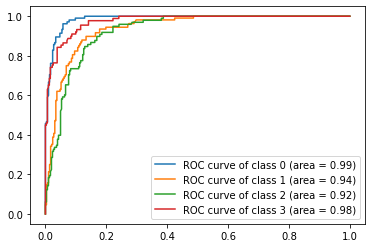
\includegraphics[width = 0.5 \textwidth]{ROCcurve/roc_random.png}}
    \subfloat[\textit{Precission-Recall curve}]{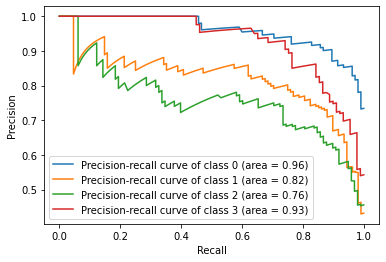
\includegraphics[width = 0.5 \textwidth]{PrecisionRecallCurve/prc_random.png}}
    \caption{Corba \textit{ROC} i \textit{Precission-Recall} del model Logístic}
    \label{fig:my_label}
\end{figure}
\hspace{-1.6em}S'observa de la corba \textit{ROC} que l'\textit{accuracy} del model és bona, ja que classifica força bé les diferents classes.\\\\
Per altra banda, de la corba \textit{Precission-Recall} s'extreu una conclusió similar a les ja trobades anteriorment (problemes en classificar la clase 1 i 2).\\\\ Per a la resta de valors s'obtenen mesures decents pel que es seguirà l'estudi del model mitjançant la recerca de la millor combinació d'hiperparàmetres possible.

\newpage
\subsubsection{Cerca dels millors hiperparàmetres}\label{bona_randomforest}
\begin{figure}[h] % Flotante "comun", sin caption, en que irán ambos
\begin{minipage}{8cm} % Minipagina para la tabla. 8 cm de ancho
 %\rowcolor{lightapricot}
\begin{center} % 0.5-b-lbfgs-l2 0.8275
    \begin{tabular}{l|l}
        \textbf{Paràmetres} & \textbf{Valors} \\\hline\hline
        \multirow{2}{*}{criterion} & gini\\
        &\cellcolor{lightapricot}entropy\\\hline
        \multirow{3}{*}{max_features} & sqrt\\
        & log2 \\ 
        & \cellcolor{lightapricot}None\\\hline
        \multirow{3}{*}{class\_weight} & \cellcolor{lightapricot}balanced\\
        &balanced\_subsample\\
        & None\\ \hline
        \multirow{2}{*}{bootstrap} & \cellcolor{lightapricot}true\\
        & false\\\hline
        \multirow{3}{*}{max\_samples} & \cellcolor{lightapricot}0.1\\
        & $\vdots$\\
        & 25\\\hline
        \multirow{5}{*}{n\_estimators} & 10\\
        & $\vdots$\\
        & \cellcolor{lightapricot}160\\
        & $\vdots$\\
        & 210\\\hline
        \multirow{5}{*}{max\_depth} & 2\\
        & $\vdots$\\
        & \cellcolor{lightapricot}11\\
        & $\vdots$\\
        & 30\\\hline
         \multirow{5}{*}{min\_samples\_split} & 2\\
        & \cellcolor{lightapricot}3\\
        & $\vdots$\\
        & 10\\
    \end{tabular}
    \caption{Hiperparàmetres model KNN}
    \label{tab:afins}
\end{center}
\end{minipage} % Fin de la minipagina de la tabla
\hspace{2em}
%\hfill % Espacio flexible para separar tabla y figura
\begin{minipage}{6.5cm} % Minipágina para la figura, 6 cm de ancho
Per a obtenir la millor precisió possible amb el RandomForest s'ha proposat trobar la combinació de paràmetres que maximitzin la \textit{accuracy}.\\ Els paràmetres i valors testejats es mostren a la taula del costat.\\\\
Els resultats de la cerca dels millors hiperparàmetres són els valors remarcats a la taula. Aquest paràmetres permeten obtenir un \textit{accuracy} del $81.5\%$ (tot i que aquest valor, en alguns casos, es pot incrementar fins a $23\%$ per fenòmens aleatoris a l'hora de generar el model).\\\\ 

\end{minipage} % Fin de la minipagina que lleva la foto
\end{figure} % Fin del entorno comun. No lleva caption
\hspace{-1.6em}S'observa una milloria però no n'és suficient en comparació al regressor logístic (\textcolor{blue}{\ref{hiper_para_log}}.\\
Com el model té un cost computacional baix i un percentatge d'encert semblant al logístic, es manté el model com a vàlid i s'analitzen les seves corbes \textit{ROC} i \textit{Precision-Recall}.\\
\hspace{-1.6em}S'analitzen ara les corbes \textit{ROC} i \textit{Precision-Recall} del model amb els millors hiperparàmetres:\\
\newpage
\begin{figure}[h]
\centering
    \subfloat[\textit{ROC curve}]{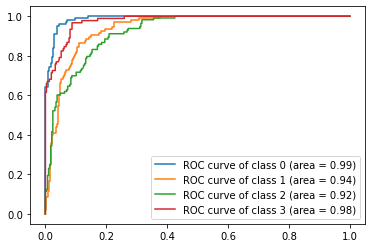
\includegraphics[width = 0.4 \textwidth]{BetterROC/ultim_roc_random.png}}
    \subfloat[\textit{Precission-Recall curve}]{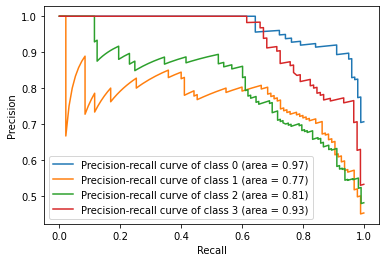
\includegraphics[width = 0.4 \textwidth]{BetterPrecision/ultim_precision_random.png}}
    \caption{Corba \textit{ROC} i \textit{Precission-Recall} del millor model \textit{Random Forest}}
    \label{fig:my_label}
\end{figure}\\
S'observa com les corbes han cambiat respecte a les obtingudes a \textcolor{blue}{\ref{ROC_Random}}, concretament com les dues corbes ha millorat en la majoria de les classes.
No obstant, s'observa el següent:
\begin{itemize}
    \item La \textit{Recall} i \textit{Precission} ha millorat en la classe 2 pero empitjorat en la classe 1
    \item Els valors son força semblants al Logístic, però no el suficient com per a classificar igual, pel que surgeix la idea de combinar els models en un ensemble. 
\end{itemize}
\newpage
\subsubsection{Resultats del classificador}\label{zona_randomforest}
Finalment, s'obté la \textit{zona de decisió} del classificador amb els millors hiperparàmetres\footnote{Els hiperparàmetres que milloren el classificador són explicats a \textcolor{blue}{\ref{bona_randomforest}}} obtinguts:\\
\begin{figure}[h]
    \centering
    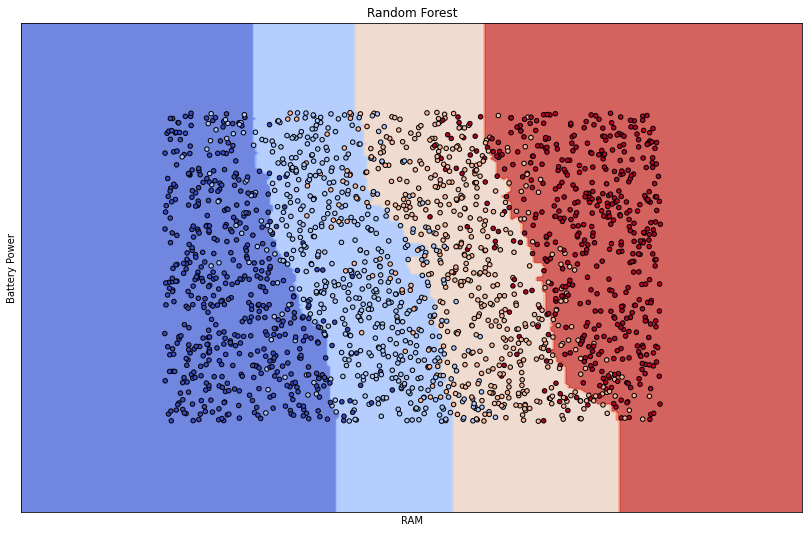
\includegraphics[width = 1\textwidth]{ZonasModelos/zona_random.png}
    \caption{Zona de decisió del millor model \textit{Random Forest} trobat}
    \label{fig:my_label}
\end{figure}\\
S'observa com la zona de decisió del millor model del Random Forest és molt similar al del model KNN (\textcolor{blue}{\ref{KNN}}) pel que arribem a la mateixa conclusió.\\\\
\newpage



\subsection{Altres metodes}
En el codi del programa s'observa com s'ha intentat millorar la predicció mitjançant ensemble methods, K-means i mètode EM, tot i així, la precisió no era prou bona pel que es van desentimar. Si es vol consultar els mètodes es recomana consultar el codi.



\newpage
\section{Resolució de les preguntes}
\subsection{Apartat B.1}
\begin{enumerate}
    \item \textbf{Quants atributs té la vostra base de dades?} 21 atributs.
    \item \textbf{Quin tipus d'atributs tens? (Númerics, temporals, categorics, binaris...)} 
    Binaris i numèrics.
    \item \textbf{Com es el target, quantes categories diferents existeixen?} 4 
    \item \textbf{Podeu veure alguna correlació entre X i y?} Com s'ha comentat en apartats anteriors \textcolor{blue}{\ref{correlacio}}, observem que hi ha una correlació entre els atributs \textit{price\_range i RAM}.
    \item \textbf{Estan balancejades les etiquetes (distribució similar entre categories)? Creus que pot afectar a la classificació la seva distribució?} Si que existeix un cert balanç, ja que la majoria són binàries o uniformes, i si que afecta a la classificació ja que si una classe és propensa a tenir un cert valor d'atribut i les altres no, ajuda a classificar aquella classe. 
\end{enumerate}

\newpage
\subsection{Apartat B.2}
\begin{enumerate}
    \item \textbf{Estàn les dades normalitzades? Caldria fer-ho?}
    Veiem que les dades no estàn normalitzades, el nostre dataset no conté dades duplicades ni anomialies del tipus \textit{NaN}. Tot i així, s'ha decidit normalitzar el dataset en casos específics, com els que s'expliquen a \textcolor{blue}{\ref{zona_decisiontree}}, \textcolor{blue}{\ref{zona_knn}}, \textcolor{blue}{\ref{zona_linearsvc}}, \textcolor{blue}{\ref{zona_logistic}}, \textcolor{blue}{\ref{zona_randomforest}}, \textcolor{blue}{\ref{zona_svc}}.

    \item \textbf{Teniu gaires dades sense informació? Els NaNs a pandas? Tingueu en compte que hi ha metodes que no els toleren durant el aprenentatge. Com afecta a la classificació si les filtrem? I si les reompliu? Com ho farieu?}
    Ens trobem en el cas, en que el nostre dataset no conté valors \textit{NaN}, però si que hi ha alguns valors amb incongruències, expliquem el tractament d'aquestes incongruències a \textcolor{blue}{\ref{exp_dataset}}.
    
    \item \textbf{Teniu dades categòriques? Quina seria la codificació amb més sentit?}
    El nostre dataset no conté dades categòriques.
    
    \item \textbf{Caldria aplicar \textit{sklearn.decomposition.PCA}? Quins beneficis o inconvenients trobarieu?}
    Hem considerat que no caldria aplicar una PCA perquè aquest s'usa quan comptem amb un gran nombre de variables amb altes correlacions, qualitat de la que no disposa el nostre dataset; exposat a \textcolor{blue}{\ref{correlacio}}. 

   \item \textbf{Es poden aplicar \textit{Polynomial Features} per millorar la classificació? En quins casos té sentit fer-ho?} No s'ha aplicat cap \textit{Polynomial Features} ja que amb les dues variables significatives \textit{RAM} i \textit{battery\_power} no té sentit aplicar combinacions lineals o polinòmiques per a obtenir atributs nous.
\end{enumerate}
\newpage
\subsection{Apartat B.3}
\begin{enumerate}
    \item \textbf{Quins models heu considerat?} Els classificadors considerats han estat exposats anteriorment a l'apartat \textcolor{blue}{\ref{classificacio}}: KNN, Logistic Regressor, Decision Tree, Random Forest, K-means, EM classifier, SVC, Linear SVC, AdaBoost Classifier, Ensemble Classifier, GridSearchCV i BayesSearchCV.
    \item \textbf{Quin creieu que serà el més precís?} El GridSearchCV, ja que té en compte tots els models estudiats anteriorment per tal de combinar-los i donar la major precisió possible, tot i que al tenir un temps de computació molt elevat que fa inviable esperar a veure els resultats, pel que cal destacar que sense tenir-lo en compte, el Logístic o SVC serien els més precisos. 
    \item \textbf{Quin serà el més ràpid?} El model logístic.
    
    \item \textbf{Seria una bona idea fer un \textit{ensemble}? Quins inconvenients creieu que pot haver-hi?} Si; ja que les tècniques ensemble fan servir diversos models per obtenir un millor resultat del que ens donaria un sol model, millorant així la precisió. L'inconvenient principal és l'alt cost computacional que implica aquesta tasca.
    
\end{enumerate}
\newpage
\subsection{Apartat B.4}
\begin{enumerate}
    \item \textbf{Per què és important cross-validar els resultats?} Per així no tenir overfitting en les dades de testeig i, per tant, millorar la precisió general del classificador.
    \item \textbf{Separa la base de dades en el conjunt de train-test. Com de fiables serán els resultats obtinguts? En quins casos serà més fiable, si tenim moltes dades d'entrenament o poques?} Les dades seran menys fiables que si disposesim de dades especialment preparades per testejar i entrenar; tot i així, la fiabilitat és suficientment alta com per a utilitzar aquest recurs. El classificador obtindrà millors prediccions com més dades d'entrenament tingui, sempre i quant en disposi de suficients per al testeig.\\ En el nostre cas s'ha dividit el dataset en un 80\% i 20\% en train i test.
    \item \textbf{Quin tipus de K-fold heu escollit? Quants conjunts heu seleccionat (quina k)? Com afecta els diferents valors de k?} S'ha utilitzat el mètode \textit{CrossValidation} de la llibreria \textit{sklearn} amb un valor de $k = 5$. S'ha observat experimentalment que en cas d'augmentar el valor de la $k$ la precisió del model únicament s'estabilitza; experimentalment s'ha trobat que el valor utilitzat, $k = 5$ és prou bo per a fer els càlculs i triga poc en obtenir-los.
    \item \textbf{És viable o convenient aplicar \textit{LeaveOneOut}?} No és viable ja que el nostre dataset no és binari i existeixen moltes similituds entre les diverses classes, pel que si només es testeja amb una dada el classificador tendirà a fer \textit{overfitting} del train i no podriem tampoc assegurar una bona classificació de les dades.
\end{enumerate}
\newpage
\subsection{Apartat B.5}
\begin{enumerate}
    \item \textbf{A teoria, hem vist el resultat d'aplicar el \textit{accuracy\_score} sobre dades no balancejades. Podríeu explicar i justificar quina de les següents mètriques será la més adient pel vostre problema? \textit{accuracy\_score}, \textit{f1\_score} o \textit{average\_precision\_score}}. S'ha utilitzat \textit{accuracy\_score} per els següents motius:
    \begin{enumerate}
        \item Les classes són equiprobables pel que no cal tenir en compte la distribució de les mateixes en el dataset.
        \item L'objectiu del classificador és etiquetar el més bé possible totes les classes, pel que hem de contar només els casos correctes respecte al total (definició \textit{accuracy\_score}).
    \end{enumerate}
    \item \textbf{Mostreu la Precisió-Recall Curve i la ROC Curve. Quina és més rellevant pel vostre dataset? Expliqueu amb les vostres paraules, la diferència entre una i altre.} Les gràfiques tant de la Precisió-Recall Curve com de la ROC Curve de cada model es troben als apartats explicats anteriorment \textcolor{blue}{\ref{ROC_DECISIONTREE}}, \textcolor{blue}{\ref{ROC_KNN}}, \textcolor{blue}{\ref{ROC_LOGISTIC}}, \textcolor{blue}{\ref{ROC_Random}}, \textcolor{blue}{\ref{ROC_SVC}}.\\
    En el nostre cas, és més important la corva ROC, degut a que el nostre dataset està balancejat i a que és més util quan es volen classificar diverses classes en representar de millor manera la precisió del mètode sense haver de binaritzar l'output.
    \item \textbf{Què mostra \textit{classification\_report}? Quina métrica us fixareu per tal de optimitzar-ne la classificació pel vostre cas?} Per fer la comparativa dels mètodes mitjançant la \textit{classification\_report} utilitzarem la mètrica \textit{f1\_score}, ja que relaciona la \textit{recall} amb la \textit{precision}, que són els dos paràmetres que s'utilitzen per a la representació de la \textit{ROC curve}.
    
\end{enumerate}
\newpage
\subsection{Apartat B.6}
\begin{enumerate}
    \item \textbf{Quines formes de buscar el millor paràmetre heu trobat? Són costoses computacionalment parlant?} Hem utilitzat un algoritme de tipus \textit{Backtracking} que és força costós computacionalment, aquesta decisió ha sigut presa degut a que altres mètodes ja implementats en la llibreria \textit{sklearn} que fan aquesta cerca dels hiperparàmetres, com pot ser el \textit{GridSerachCV}, triguen massa en obtenir la millor combinació de paràmetres possible. De la nostra manera, si bé es més tediós, obtenim mica en mica la millor combinació i podem anant estudiant els paràmetres que obtenim per veure si té sentit o si podem utilitzar algún altre algoritme que s'ajusti millor.
    \item \textbf{Si disposem de recursos limitats (per exemple, un PC durant 1 hora) quin dels dos mètodes creieu que obtindrà millor resultat final?} Seria bastant més eficaç utilitzar el \textit{GridSearchCV} ja que la implementació propia de l'algoritme de cerca es bastant ineficient.
    \item \textbf{Existeixen altres mètodes de búsqueda més eficients (\textit{scikit-optimize})?} Existeixen el \textit{BayessianSearchCV} i el \textit{Tunning} de \textit{skopt} entre altres que són més eficients. S'ha testejat el \textit{GridSearchCV} i el \textit{BayesianSearchCV} en el codi entregat tot i que no s'han utilitzat els seus resultats a l'hora de trobar el millor classificador (ja que amb el nostre propi algoritme obteníem precisions semblants amb un temps d'execució relativament baix) i no s'ha inclòs l'ouput del programa quan s'executava el fragment de codi mencionat degut a la redundància dels resultats obtinguts amb el nostre propi mètode.
\end{enumerate}
\newpage
\section{Conclusions}
Concluïm el proces mostrant una taula de eficiencies (model i precisió) amb els millors models obtinguts.
\begin{center} % 0.5-b-lbfgs-l2 0.8275
    \begin{tabular}{l|l}
        \textbf{model} & \textbf{precisió} \\\hline\hline
        KNN & 82.5\% \\ \hline
        \rowcolor{lightapricot}
        SVC & 84\%\\ \hline
        RandomForest & 81.5\%
        Logistic & 82.75\% \\ \hline
        SVC_linear & 76.25\%\\ \hline
        DecisionTree & 81.5\%\\
    \end{tabular}
    \caption{Hiperparàmetres model KNN}
    \label{tab:afins}
\end{center}
Concluïm doncs que el millor model és el SVC amb els hiperparàmetres explicats a \textcolor{blue}{\ref{hiper_par_SVC}}.\\
Tot i així, també es recomana utilitzar el Logistic en ja que no hem obtingut resultats amb tanta variança.


\newpage
\section{Annex}
\subsection{Histogrames}\label{histogrames}

\begin{figure}[h]
 \centering
  \subfloat[\textit{Battery Power}]{
    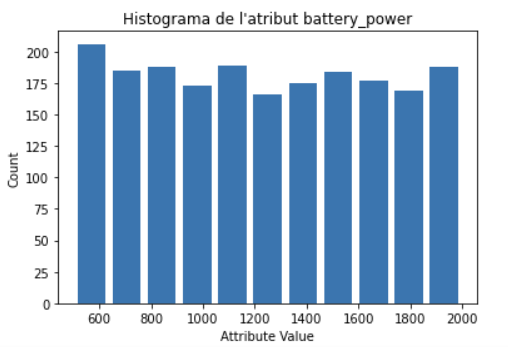
\includegraphics[width=0.3\textwidth]{Histogramas/bt_power.png}}
  \subfloat[\textit{Blue}]{
    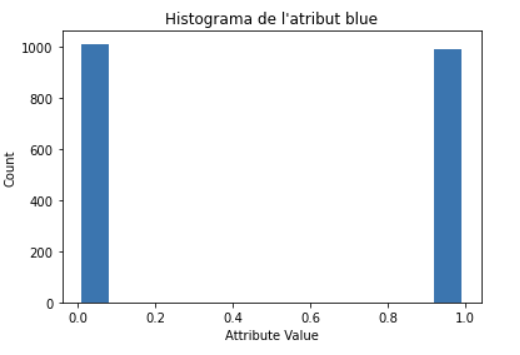
\includegraphics[width=0.3\textwidth]{Histogramas/blue.png}}
  \subfloat[\textit{Clock Speed}]{
    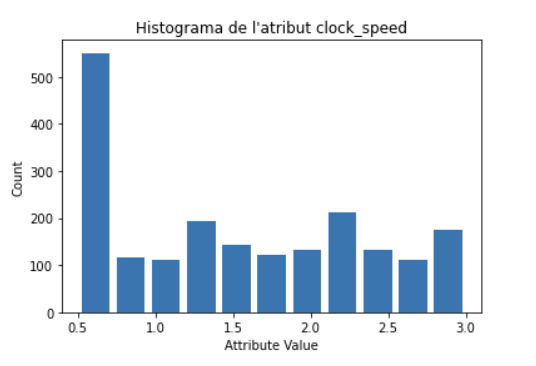
\includegraphics[width=0.3\textwidth]{Histogramas/clock_speed.png}}
\end{figure}
\begin{figure}[h]
 \centering
  \subfloat[\textit{Dual Sim}]{
    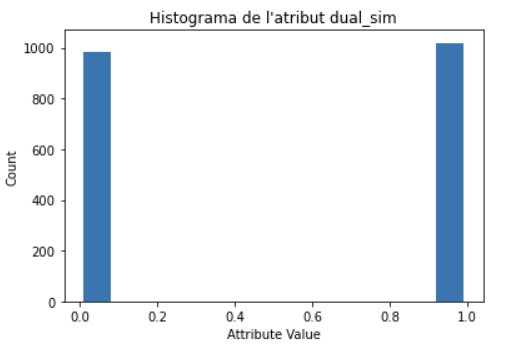
\includegraphics[width=0.3\textwidth]{Histogramas/dual_sim.png}}
  \subfloat[\textit{Frontal Camera}]{
    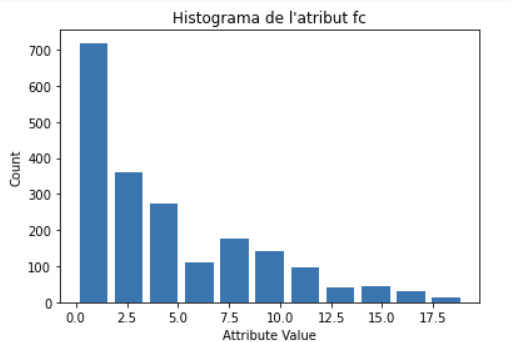
\includegraphics[width=0.3\textwidth]{Histogramas/fc.png}}
  \subfloat[\textit{4G}]{
    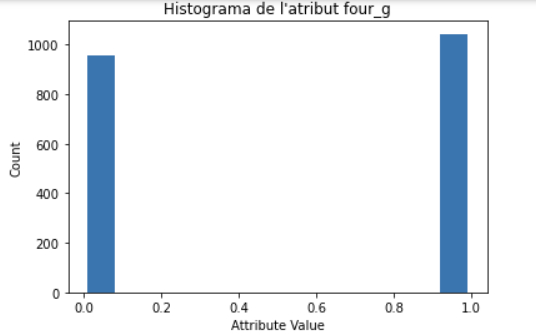
\includegraphics[width=0.3\textwidth]{Histogramas/4g.png}}
\end{figure}
\begin{figure}[h]
 \centering
  \subfloat[\textit{Intern Memory}]{
    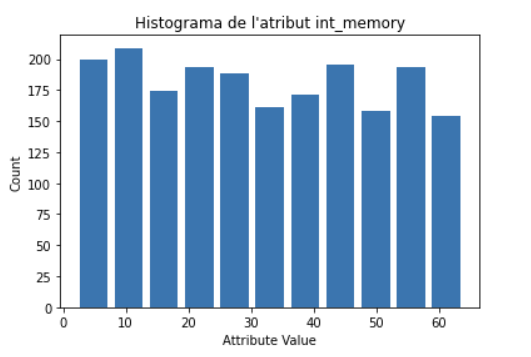
\includegraphics[width=0.3\textwidth]{Histogramas/int_memory.png}}
  \subfloat[\textit{Mobile Depth}]{
    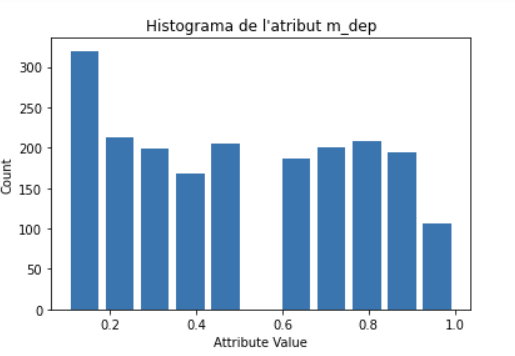
\includegraphics[width=0.3\textwidth]{Histogramas/m_dep.png}}
  \subfloat[\textit{Number Cores}]{
    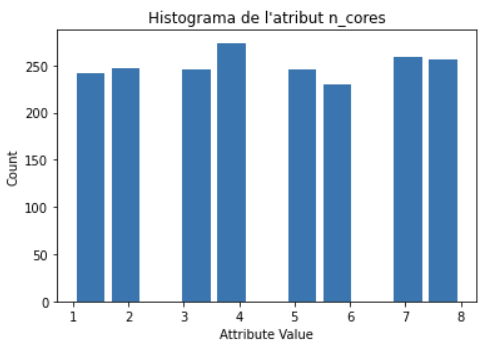
\includegraphics[width=0.3\textwidth]{Histogramas/n_cores.png}}
\end{figure}
\newpage
\begin{figure}[h]
 \centering
  \subfloat[\textit{PC}]{
    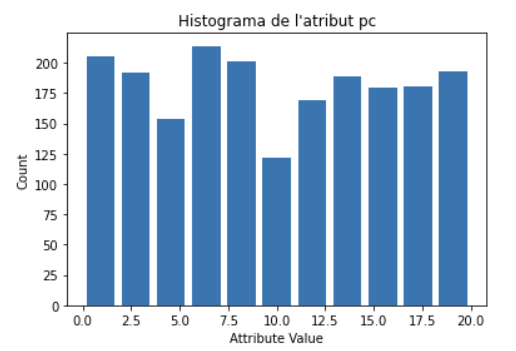
\includegraphics[width=0.3\textwidth]{Histogramas/pc.png}}
  \subfloat[\textit{Px Height}]{
    \includegraphics[width=0.3\textwidth]{Histogramas/px_weight.png}}
  \subfloat[\textit{Px Width}]{
    \includegraphics[width=0.3\textwidth]{Histogramas/px_width.png}}
\end{figure}
\begin{figure}[h]
 \centering
  \subfloat[\textit{RAM}]{
    \includegraphics[width=0.3\textwidth]{Histogramas/ram.png}}
  \subfloat[\textit{Screen Height}]{
    \includegraphics[width=0.3\textwidth]{Histogramas/sc_h.png}}
  \subfloat[\textit{Screen Width}]{
    \includegraphics[width=0.3\textwidth]{Histogramas/sc_w.png}}
\end{figure}
\begin{figure}[h]
 \centering
  \subfloat[\textit{Talk Time}]{
    \includegraphics[width=0.3\textwidth]{Histogramas/tlk_t.png}}
  \subfloat[\textit{3G}]{
    \includegraphics[width=0.3\textwidth]{Histogramas/3g.png}}
  \subfloat[\textit{Touch Screen}]{
    \includegraphics[width=0.3\textwidth]{Histogramas/touch_screen.png}}
\end{figure}
\newpage
\begin{figure}[h]
 \centering
  \subfloat[\textit{Wifi}]{
    \includegraphics[width=0.3\textwidth]{Histogramas/wifi.png}}
  \subfloat[\textit{Price Range}]{
    \includegraphics[width=0.3\textwidth]{Histogramas/price_range.png}}
\end{figure}
\newpage

\subsection{Correlacions amb \textit{price\_range}} \label{scatter}

\begin{figure}[h]
 \centering
  \subfloat[\textit{Battery Power}]{
    \includegraphics[width=0.3\textwidth]{Scatterplots/battery_price.png}}
  \subfloat[\textit{Blue}]{
    \includegraphics[width=0.3\textwidth]{Scatterplots/blue_price.png}}
  \subfloat[\textit{Clock Speed}]{
    \includegraphics[width=0.3\textwidth]{Scatterplots/clock_price.png}}
\end{figure}
\begin{figure}[h]
 \centering
  \subfloat[\textit{Dual Sim}]{
    \includegraphics[width=0.3\textwidth]{Scatterplots/sim_price.png}}
  \subfloat[\textit{Frontal Camera}]{
    \includegraphics[width=0.3\textwidth]{Scatterplots/fc_price.png}}
  \subfloat[\textit{4G}]{
    \includegraphics[width=0.3\textwidth]{Scatterplots/4g_price.png}}
\end{figure}
\begin{figure}[h]
 \centering
  \subfloat[\textit{Intern Memory}]{
    \includegraphics[width=0.3\textwidth]{Scatterplots/memory_price.png}}
  \subfloat[\textit{Mobile Depth}]{
    \includegraphics[width=0.3\textwidth]{Scatterplots/mdep_price.png}}
  \subfloat[\textit{Number Cores}]{
    \includegraphics[width=0.3\textwidth]{Scatterplots/ncores_price.png}}
\end{figure}
\newpage
\begin{figure}[h]
 \centering
  \subfloat[\textit{PC}]{
    \includegraphics[width=0.3\textwidth]{Scatterplots/pc_price.png}}
  \subfloat[\textit{Px Height}]{
    \includegraphics[width=0.3\textwidth]{Scatterplots/pxheight_price.png}}
  \subfloat[\textit{Px Width}]{
    \includegraphics[width=0.3\textwidth]{Scatterplots/pxwidth_price.png}}
\end{figure} 
\begin{figure}[h]
 \centering
  \subfloat[\textit{RAM}]{
    \includegraphics[width=0.3\textwidth]{Scatterplots/ram_price.png}}
  \subfloat[\textit{Screen Height}]{
    \includegraphics[width=0.3\textwidth]{Scatterplots/sch_price.png}}
  \subfloat[\textit{Screen Width}]{
    \includegraphics[width=0.3\textwidth]{Scatterplots/scw_price.png}}
\end{figure}
\begin{figure}[h]
 \centering
  \subfloat[\textit{Talk Time}]{
    \includegraphics[width=0.3\textwidth]{Scatterplots/talktime_price.png}}
  \subfloat[\textit{3G}]{
    \includegraphics[width=0.3\textwidth]{Scatterplots/3g_price.png}}
  \subfloat[\textit{Touch Screen}]{
    \includegraphics[width=0.3\textwidth]{Scatterplots/touchscreen_price.png}}
\end{figure}
\newpage
\begin{figure}[h]
 \centering
  \subfloat[\textit{Wifi}]{
    \includegraphics[width=0.3\textwidth]{Scatterplots/wifi_price.png}}
  \subfloat[\textit{Price Range}]{
    \includegraphics[width=0.3\textwidth]{Scatterplots/price_price.png}}
\end{figure}

\newpage
\subsection{Cerca hiperparàmetres}
\subsubsection{Logistic Regressor}\label{hiper_logistic}
\begin{figure}[h]
    \includegraphics[width=0.7\textwidth]{LosQueFaltan/crosval_logistic.png}
\end{figure}
\newpage
\subsubsection{K-Nearest Neighbors}\label{hiper_knn}
\begin{figure}[h]
 \captionsetup[subfigure]{labelformat=empty}
 \centering
    \subfloat[Búsqueda dels millors \textit{weights} i \textit{algorithm}]{
    \includegraphics[width=0.45\textwidth]{LosQueFaltan/crosval_knn.png}}
\end{figure}
\begin{figure}[h]
 \captionsetup[subfigure]{labelformat=empty}
 \centering
    \subfloat[Búsqueda de la millor \textit{p}]{
    \includegraphics[width=0.45\textwidth]{LosQueFaltan/crosval_knn2.png}}
\end{figure}
\begin{figure}[h]
 \captionsetup[subfigure]{labelformat=empty}
 \centering
    \subfloat[Búsqueda del millor \textit{n\_neighbors}]{
    \includegraphics[width=0.45\textwidth]{LosQueFaltan/crosval_knn3.png}}
\end{figure}
\newpage
\subsubsection{Support Vector Classification}\label{hiper_svc}
\begin{figure}[h]
 \centering
    \includegraphics[width=0.7\textwidth]{LosQueFaltan/crosval_svc.png}
\end{figure}

\newpage

\subsubsection{Linear Support Vector Classification}\label{hiper_linearsvc}
\begin{figure}[h]
 \captionsetup[subfigure]{labelformat=empty}
 \centering
    \subfloat[Búsqueda dels millors \textit{class\_weight}, \textit{multi\_class}, \textit{loss} i \textit{penalty}]{
    \includegraphics[width=0.45\textwidth]{LosQueFaltan/crosval_linear.png}}
\end{figure}
\begin{figure}[h]
 \captionsetup[subfigure]{labelformat=empty}
 \centering
    \subfloat[Búsqueda del millor \textit{max\_iter}]{
    \includegraphics[width=0.45\textwidth]{LosQueFaltan/crosval_linear2.png}}
\end{figure}
\begin{figure}[h]
 \captionsetup[subfigure]{labelformat=empty}
 \centering
    \subfloat[Búsqueda de \textit{max\_iter} acotada]{
    \includegraphics[width=0.45\textwidth]{LosQueFaltan/crosval_linear3.png}}
\end{figure}
\newpage

\subsubsection{Decision Tree Classificator}\label{hiper_decisiontree}
\begin{figure}[h]
\captionsetup[subfigure]{labelformat=empty}
 \centering
    \subfloat[Búsqueda dels \textit{criterion}, \textit{max\_features} i \textit{splitter}]{
    \includegraphics[width=0.45\textwidth]{LosQueFaltan/crosval_decisiontree.png}}
\end{figure}
\begin{figure}[h]
 \captionsetup[subfigure]{labelformat=empty}
 \centering
    \subfloat[Búsqueda del millor \textit{max\_depth}]{
    \includegraphics[width=0.45\textwidth]{LosQueFaltan/crosval_decisiontree2.png}}

\end{figure}
\begin{figure}[h]
 \captionsetup[subfigure]{labelformat=empty}
 \centering
    \subfloat[Búsqueda del millor \textit{min\_samples\_split}]{
    \includegraphics[width=0.45\textwidth]{LosQueFaltan/crosval_decisiontree3.png}}
\end{figure}
\newpage
\subsubsection{Random Forest Classificator}\label{hiper_randomforest}
\begin{figure}[h]
 \captionsetup[subfigure]{labelformat=empty}
 \centering
    \subfloat[Búsqueda dels \textit{criterion}, \textit{max\_features} i  \textit{class\_weight}]{
    \includegraphics[width=0.4\textwidth]{LosQueFaltan/crosval_randomforest1.png}}
    \subfloat[Búsqueda del millor \textit{max\_samples}]{\includegraphics[width=0.4\textwidth]{LosQueFaltan/crosval_randomforest2.png}}
\end{figure}
\begin{figure}[h]
 \captionsetup[subfigure]{labelformat=empty}
 \centering
    \subfloat[Búsqueda del millor \textit{n\_estimators}]{
     \includegraphics[width=0.4\textwidth]{LosQueFaltan/crosval_randomforest3.png}}
    \subfloat[Búsqueda del millor \textit{n\_estimators} acotada]{\includegraphics[width=0.4\textwidth]{LosQueFaltan/crosval_randomforest4.png}}
\end{figure}
\begin{figure}[h]
 \captionsetup[subfigure]{labelformat=empty}
 \centering
    \subfloat[Búsqueda de la millor \textit{max\_depth}]{
    \includegraphics[width=0.4\textwidth]{LosQueFaltan/crosval_randomforest5.png}}
    \subfloat[Búsqueda del millor \textit{min\_samples\_split}]{\includegraphics[width=0.4\textwidth]{LosQueFaltan/crosval_randomforest6.png}}
\end{figure}

\newpage
\subsubsection{AdaBoost Classificator}\label{hiper_ada}
\begin{figure}[h]
 \captionsetup[subfigure]{labelformat=empty}
 \centering
    \subfloat[Búsqueda del millor \textit{base\_estimator}]{
    \includegraphics[width=0.4\textwidth]{LosQueFaltan/crosval_ada.png}}
    \subfloat[Búsqueda del millor \textit{algorithm}]{\includegraphics[width=0.4\textwidth]{LosQueFaltan/crosval_ada2.png}}
\end{figure}
\begin{figure}[h]
 \captionsetup[subfigure]{labelformat=empty}
 \centering
    \subfloat[Búsqueda del millor \textit{learning\_rat}e]{
    \includegraphics[width=0.4\textwidth]{LosQueFaltan/crosval_ada3.png}}
    \subfloat[Búsqueda del millor \textit{n\_estimators}]{\includegraphics[width=0.4\textwidth]{LosQueFaltan/crosval_ada4.png}}
\end{figure}
\end{document}
